\documentclass[12pt,a4paper]{article}

%--------------------------------------------------------------
% CODIFICACION, FUENTE E IDIOMA
%   Con inputenc[utf8] + fontenc[T1] + babel[spanish] puedes
%   escribir tildes y enes directamente: á é í ó ú ñ ¿ ¡
%--------------------------------------------------------------
\usepackage[utf8]{inputenc}
\usepackage[T1]{fontenc}
\usepackage[spanish,es-tabla]{babel}
\usepackage{textcomp}
\usepackage{helvet}
\renewcommand{\familydefault}{\sfdefault}
\usepackage{microtype}
\usepackage{pdflscape}

%--------------------------------------------------------------
% GEOMETRIA DE PAGINA
%--------------------------------------------------------------
\usepackage[a4paper,
            top=2.5cm, bottom=2.5cm,
            left=2.5cm, right=2.5cm,
            headheight=15pt]{geometry}
%--------------------------------------------------------------
% COLORES
%--------------------------------------------------------------
\usepackage[table]{xcolor}
\definecolor{BlueHeader}{HTML}{1F4E79}   % Azul oscuro cabeceras
\definecolor{MediumBlue}{HTML}{2E75B6}   % Azul medio subtitulos
\definecolor{LightBlue}{HTML}{D6E4F0}    % Azul claro fondos
\definecolor{BlueCell}{HTML}{BDD7EE}     % Azul celda ID hitos
\definecolor{LightGray}{HTML}{F2F2F2}    % Gris filas pares
\definecolor{DarkGray}{HTML}{595959}     % Gris oscuro textos
\definecolor{GreenOK}{HTML}{1F7A1F}      % Verde completado

%--------------------------------------------------------------
% TABLAS
%--------------------------------------------------------------
\usepackage{booktabs}
\usepackage{tabularx}
\usepackage{multirow}
\usepackage{array}
\usepackage{colortbl}
\usepackage{makecell}
\usepackage{ragged2e}

%--------------------------------------------------------------
% GRAFICOS Y GEOMETRIA
%--------------------------------------------------------------
\usepackage{graphicx}
\usepackage{tikz}

%--------------------------------------------------------------
% SECCIONES
%--------------------------------------------------------------
\makeatletter

% SECTION: colorbox azul con numero y titulo dentro
\newcommand{\secfmt}[1]{%
  \noindent\colorbox{BlueHeader}{%
    \parbox[b]{\dimexpr\linewidth-2\fboxsep}{%
      \vspace{5pt}%
      \textcolor{white}{\large\bfseries #1}%
      \vspace{5pt}%
    }%
  }\par\vspace{4pt}%
}

\renewcommand\section{%
  \@ifstar\section@star\section@nostar
}
\newcommand\section@nostar[1]{%
  \refstepcounter{section}%
  \addcontentsline{toc}{section}{\protect\numberline{\thesection}#1}%
  \secfmt{\thesection.\enspace #1}%
}
\newcommand\section@star[1]{%
  \secfmt{#1}%
}

% SUBSECTION: texto azul, sin raya
\newcommand{\subsecfmt}[1]{%
  {\large\bfseries\color{MediumBlue}#1}%
  \par\vspace{2pt}%
}

\renewcommand\subsection{%
  \@ifstar\subsection@star\subsection@nostar
}
\newcommand\subsection@nostar[1]{%
  \refstepcounter{subsection}%
  \addcontentsline{toc}{subsection}{\protect\numberline{\thesubsection}#1}%
  \vspace{10pt}%
  \subsecfmt{\thesubsection.\enspace #1}%
  \vspace{2pt}%
}
\newcommand\subsection@star[1]{%
  \vspace{10pt}\subsecfmt{#1}\vspace{2pt}%
}

% SUBSUBSECTION: bold azul sin numero
\renewcommand\subsubsection{\@startsection{subsubsection}{3}{\z@}%
  {-1.5ex \@plus -.3ex}{0.2ex}%
  {\normalsize\bfseries\color{MediumBlue}}}

\makeatother

%--------------------------------------------------------------
% LISTAS
%--------------------------------------------------------------
\usepackage{enumitem}
\setlist[itemize,1]{%
  label=\textcolor{MediumBlue}{\textbullet},
  leftmargin=1.6em, itemsep=2pt, topsep=4pt, parsep=0pt}
\setlist[itemize,2]{%
  label=\textcolor{DarkGray}{$\circ$},
  leftmargin=2.8em, itemsep=1pt, topsep=2pt, parsep=0pt}

%--------------------------------------------------------------
% ENCABEZADOS Y PIES
%--------------------------------------------------------------
\usepackage{fancyhdr}
\pagestyle{fancy}
\fancyhf{}
\renewcommand{\headrulewidth}{0pt}
\fancyfoot[C]{\small\thepage}

%--------------------------------------------------------------
% HIPERLINKS
%--------------------------------------------------------------
\usepackage[hidelinks,
            pdftitle={Entrega 3 - Proyecto REC},
            pdfauthor={LAR UPM}]{hyperref}

%--------------------------------------------------------------
% COMANDOS DE UTILIDAD
%--------------------------------------------------------------
\usepackage{parskip}
\setlength{\parskip}{6pt}
\setlength{\parindent}{0pt}

\usepackage{amssymb}  % \checkmark

% Filas alternas en tablas
\newcommand{\rowA}{\rowcolor{LightGray}}
\newcommand{\rowB}{\rowcolor{white}}

% Encabezado de paquete de trabajo (WP)
\newcommand{\mywphead}[1]{%
  \vspace{8pt}%
  \noindent{\normalsize\bfseries\color{MediumBlue}#1}%
  \par\vspace{3pt}}

%--------------------------------------------------------------
% PAQUETES PARA LAS SECCIONES 2 Y 3 (descripcion del sistema)
%--------------------------------------------------------------
\usepackage{amsmath,amsfonts}
\usepackage{float}              % entorno [H]
\usepackage{listings}
\usepackage{pgfplots}
\pgfplotsset{compat=1.17}
\usetikzlibrary{arrows.meta,positioning,calc,shapes.geometric,fit,backgrounds}

% Colorines para los diagramas de vision/HMI
\definecolor{recazul}{HTML}{2E75B6}
\definecolor{recverde}{HTML}{4CAF50}
\definecolor{recnaranja}{HTML}{E07B39}

% Comando \code para nombres de ficheros, nodos y topicos
\newcommand{\code}[1]{%
  \begingroup
  \def\_{\char`_\penalty0 }%   permite cortar tras "_"
  \def\/{\char`/\penalty0 }%   permite cortar tras "/"
  \texttt{\small #1}%
  \endgroup}

\setlength{\emergencystretch}{5em}
% Estilos de nodos para los diagramas TikZ
\tikzset{
  paso/.style     = {draw, rounded corners, align=center, font=\scriptsize,
                     fill=LightBlue, minimum height=8mm, minimum width=26mm,
                     inner sep=3pt},
  decision/.style = {draw, diamond, aspect=2, align=center, font=\scriptsize,
                     fill=BlueCell, inner sep=1pt},
  estado/.style   = {draw, rounded corners, align=center, font=\scriptsize,
                     fill=LightGray, minimum height=8mm, minimum width=24mm},
  blk/.style      = {draw, rounded corners, align=center, font=\scriptsize,
                     fill=LightGray, minimum height=8mm},
  blkpy/.style    = {draw, rounded corners, align=center, font=\scriptsize,
                     fill=recverde!18, minimum height=9mm},
  blkcpp/.style   = {draw, rounded corners, align=center, font=\scriptsize,
                     fill=recazul!18, minimum height=8mm},
  blkext/.style   = {draw, rounded corners, align=center, font=\scriptsize,
                     fill=recnaranja!18, minimum height=8mm},
  blkhmi/.style   = {draw, rounded corners, align=center, font=\scriptsize,
                     fill=MediumBlue!20, minimum height=10mm},
  flecha/.style   = {-{Latex}, thick},
  flechad/.style  = {-{Latex}, thick, dashed},
  lbl/.style      = {font=\scriptsize\itshape, fill=white, inner sep=1pt},
  nota/.style     = {font=\scriptsize, text=DarkGray},
}

% Estilo de listings para fragmentos de codigo
\lstset{
  basicstyle=\ttfamily\footnotesize,
  breaklines=true,
  columns=fullflexible,
  keepspaces=true,
  frame=single,
  rulecolor=\color{BlueCell},
  backgroundcolor=\color{LightGray},
  xleftmargin=4pt, xrightmargin=4pt,
  aboveskip=6pt, belowskip=6pt,
}

%==============================================================
\begin{document}
%==============================================================

%--------------------------------------------------------------
% PORTADA
%--------------------------------------------------------------
% PORTADA
%--------------------------------------------------------------

\begin{titlepage}
    \begin{center}
        

        \IfFileExists{EscudoUPM.png}{
            
\includegraphics[width=4cm]{EscudoUPM.png}
        }{
            \framebox[3cm]{\parbox[c][4cm]{3.5cm}{\centering \tiny EscudoUPM.png \\ (Place file in folder)}}
        }
        
        \vspace{0.5cm}
        
        \textsc{\LARGE Universidad Politécnica de Madrid}\\[0.35cm]
        \textsc{\Large Escuela Técnica Superior de Ingenieros Industriales}\\[1cm]

        \textsc{\Large Máster en Robótica y Automática}\\[0.35cm]
        \textsc{\large Laboratorio de Robótica y Automática}\\[1.0cm]

        % --- TÍTULO DEL PROYECTO ---

        \rule{\linewidth}{0.3mm} \\[0.35cm]
        { \huge \bfseries  Clasificación de tapones plásticos (REC)\\[0.35cm] }
        \rule{\linewidth}{0.3mm} \\[1.5cm]
        
        % --- AUTORES Y PROFESOR ---
        \begin{minipage}{0.5\textwidth}
            \begin{center} \large
                \emph{Autores:}\\
                \textbf{Silvia Ochando Valero}\\
                \textbf{Asil Arnous}\\
                \textbf{Delia Martinez Fernandez}\\
                \textbf{Ruth A. Bastidas Alva}\\
        	\textbf{}\\
            \end{center}
        \end{minipage}
        \hfill % Espacio flexible entre columnas
        \begin{minipage}{0.4\textwidth}
            % Alinear a la izquierda para que el texto se vea natural
            \begin{center} \large 
                \emph{Profesores:}\\
                \textbf{Jaime Del Cerro}\\               
            \end{center}
        \end{minipage}
        \vfill

        % --- LOGO INFERIOR (Escuela/Departamento) ---
        \IfFileExists{Logo-Nombre-Industriales.png}{
            
\includegraphics[width=4cm]{Logo-Nombre-Industriales.png}
        }{
             \framebox[3cm]{\parbox[c][2cm]{5cm}{\centering \tiny Logo-Nombre-Industriales.png \\ (Place file in folder)}}
        }

        \vspace{0.2cm}

        % --- FECHA ---
        {\large Madrid, \today}

    \end{center}
\end{titlepage}

\newpage

%--------------------------------------------------------------
% INDICE
%--------------------------------------------------------------
\thispagestyle{fancy}
{%
  \large\bfseries ÍNDICE%
  \par\vspace{4pt}%
}
\vspace{4pt}
\setcounter{tocdepth}{2}
\makeatletter\@starttoc{toc}\makeatother
\newpage

%==============================================================
% 1. SEGUIMIENTO DEL PROYECTO
%==============================================================
\section{Seguimiento del proyecto}

En esta tercera y última entrega se presenta el estado final del Proyecto REC: Clasificación de Tapones de Plásticos. A continuación se recogen los objetivos previstos para esta fase, los objetivos alcanzados, las acciones correctivas aplicadas durante el desarrollo y la planificación temporal definitiva del proyecto, incluyendo la EDP actualizada, los hitos finales y la asignación real de horas por participante y sub-equipo.

%--------------------------------------------------------------
\subsection{Objetivos previstos}
%--------------------------------------------------------------

Los objetivos planificados para esta tercera entrega correspondían a la finalización y validación
integral del sistema, abarcando las fases de integración y validación (WP-500 y WP-600), la
depuración final del sistema de visión (WP-300), la optimización de tiempos de ciclo en
manipulación (WP-400) y el cierre documental y de gestión del proyecto (WP-100 y WP-200).
A continuación se detallan los objetivos por paquete de trabajo:

\mywphead{WP-100 -- Gestión del proyecto}
\begin{itemize}
  \item \textbf{103} -- Especificación de requisitos del sistema: consolidación final del documento de
        requisitos funcionales y técnicos.
  \item \textbf{104} -- Coordinación de actividades de los sub-equipos: coordinación final durante las
        fases de integración y validación.
  \item \textbf{107} -- Control e integración de los cambios: cierre del repositorio con control de
        versiones y trazabilidad completa.
\end{itemize}

\mywphead{WP-200 -- Diseño de la interfaz y arquitectura del sistema}
\begin{itemize}
  \item \textbf{201} -- Diseño de la arquitectura de software: definición final de la estructura de
        nodos ROS2 (Humble) y de los tópicos de comunicación entre los paquetes \texttt{lra\_vision},
        \texttt{rec\_vision}, \texttt{ur3\_vision\_control} y \texttt{lra\_hmi}.
  \item \textbf{202} -- Diseño de la interfaz de usuario: implementación de la HMI gráfica en PyQt5
        (\texttt{lra\_hmi}) como lanzador y panel de supervisión del sistema completo.
  \item \textbf{203} -- Definición de protocolos de comunicación y lógica de control: establecimiento
        de las reglas de arranque, parada y parada de emergencia entre la HMI y el resto de nodos.
\end{itemize}

\mywphead{WP-300 -- Sistema de Visión}
\begin{itemize}
  \item \textbf{308} -- Depuración final del algoritmo: ajuste de parámetros de detección y mejora de la robustez del sistema de visión antes de
        la integración final.
\end{itemize}

\mywphead{WP-400 -- Manipulación y Efector}
\begin{itemize}
  \item \textbf{405} -- Optimización de tiempos de ciclo: ajuste final de aceleraciones, candidatos de
        orientación y aproximación para minimizar el tiempo de ejecución de cada ciclo de pick~\& place.
\end{itemize}

\mywphead{WP-500 -- Integración}
\begin{itemize}
  \item \textbf{501} -- Conexión de red y comunicación ROS2: puesta en marcha del driver del UR3e y
        del intercambio de mensajes entre los nodos de visión, control y HMI.
  \item \textbf{502} -- Integración del sistema de visión con el sistema de manipulación: integración
        de coordenadas (\texttt{/ur3/target\_point}) y caja asignada (\texttt{/tapones/caja\_asignada})
        con el nodo de manipulación del UR3e.
  \item \textbf{503} -- Algoritmo de lógica de clasificación: clasificación de cada tapón por color
        mediante K-Means y asignación a una de las N~cajas de descarga (configurable 1-6, por defecto~3).
  \item \textbf{504} -- Sincronización y control de flujo: implementación del \textit{gating} por
        \texttt{/vision\_enable} para evitar lecturas de visión mientras el robot está en movimiento.
  \item \textbf{505} -- Protocolo de gestión de excepciones: rutinas de seguridad para objetivos fuera
        de alcance, fallos de transformación TF y parada de emergencia desde la HMI.
\end{itemize}

\mywphead{WP-600 -- Validación}
\begin{itemize}
  \item \textbf{601} -- Definición de las pruebas de validación del sistema.
  \item \textbf{602} -- Validación estadística de clasificación por color: ejecución de ciclos
        completos para verificar la robustez del algoritmo de clasificación.
  \item \textbf{603} -- Verificación de seguridad y exclusión de colisiones: validación de que el
        planificador rechaza trayectorias que comprometan la integridad del entorno.
  \item \textbf{604} -- Verificación de tiempos de ciclo: medición de tiempos finales de ejecución
        para comprobar el cumplimiento de las especificaciones.
\end{itemize}

%--------------------------------------------------------------
\subsection{Objetivos alcanzados}
%--------------------------------------------------------------

Al cierre del proyecto, la totalidad de los objetivos planificados han sido alcanzados.
El sistema completo de clasificación de tapones plásticos está operativo, integrando los módulos de
visión, manipulación, integración e interfaz de usuario sobre la arquitectura ROS2 Humble.

\mywphead{WP-100 -- Gestión del proyecto}
\begin{itemize}
  \item \textbf{Tareas completadas: 101, 102, 103, 104, 105, 106, 107.}
  \begin{itemize}
    \item La documentación final ha sido elaborada satisfactoriamente, incluyendo las tres entregas,
          los vídeos de seguimiento y el vídeo de demostración final.
    \item El repositorio GitHub ha sido cerrado con control de versiones completo y los README de cada
          paquete actualizados.
    \item Todas las reuniones de coordinación han sido realizadas.
  \end{itemize}
\end{itemize}
\clearpage
\mywphead{WP-200 -- Diseño de la interfaz y arquitectura del sistema}
\begin{itemize}
  \item \textbf{Tareas completadas: 201, 202, 203.}
  \begin{itemize}
    \item La arquitectura se ha estructurado en cuatro paquetes ROS2 con responsabilidades separadas:
          \texttt{lra\_vision} (cámara y calibración), \texttt{rec\_vision} (detección y clasificación),
          \texttt{ur3\_vision\_control} (manipulación) y \texttt{lra\_hmi} (interfaz de usuario).
    \item La Interfaz Gráfica de Usuario (HMI) en PyQt5 ha sido implementada como lanzador único del
          sistema, sustituyendo el arranque manual por terminales. Permite iniciar, detener y reiniciar
          cada subsistema, dispone de parada de emergencia, monitor de conexión del UR3e, contadores por
          caja y totales, lectura de ángulos articulares y visualización de la cámara en directo.
    \item Los protocolos de comunicación entre la HMI y el resto de nodos han quedado definidos y
          validados.
  \end{itemize}
\end{itemize}

\mywphead{WP-300 -- Sistema de Visión}
\begin{itemize}
  \item \textbf{Tareas completadas: 301, 302, 303, 304, 305, 306, 307, 308.}
  \begin{itemize}
    \item El algoritmo de visión ha sido depurado y optimizado en su versión final. La detección de
          tapones mediante la Transformada de Hough Circular sobre la ROI de la caja de trabajo
          (segmentada en HSV) funciona de forma robusta y estable.
    \item La clasificación por color se realiza con K-Means: un nodo calibrador (\texttt{color\_calibrator\_node})
          se ejecuta una sola vez al inicio, agrupa los tapones y publica de forma persistente
          los centros HSV de cada caja, que el nodo detector consume para asignar cada tapón.
    \item El número de cajas es configurable (de~1 a~6, por defecto~3) y se fija desde la interfaz de
          usuario antes de arrancar la clasificación.
    \item El mecanismo de selección estable por análisis multifotograma (30~frames con \textit{clustering}
          espacial) minimiza los falsos positivos, y se ha fijado una semilla aleatoria para garantizar
          la reproducibilidad de la detección y la clasificación entre arranques.
    \item La transformación de coordenadas píxel a espacio~3D del robot se realiza con el modelo
          \textit{pinhole} (corrección de distorsión con \texttt{undistortPoints}) y la intersección del
          rayo con el plano de la mesa mediante el árbol de transformaciones TF2.
  \end{itemize}
\end{itemize}

\mywphead{WP-400 -- Manipulación y Efector}
\begin{itemize}
  \item \textbf{Tareas completadas: 401, 402, 403, 404, 405.}
  \begin{itemize}
    \item El efector final validado es una ventosa, montada como herramienta del TCP del UR3e.
          La detección de visión ya no calcula el diámetro del tapón, al no requerirse para la recogida
          por vacío.
    \item La secuencia de pick~\& place
          (\textit{Home} $\rightarrow$ \textit{Aproximación} $\rightarrow$ \textit{Pick} $\rightarrow$
          \textit{Retreat} $\rightarrow$ \textit{Clasificación} $\rightarrow$ \textit{Drop} $\rightarrow$
          \textit{Home})
          funciona de forma fiable y continua para todas las cajas configuradas.
    \clearpage      
    \item La optimización de tiempos de ciclo se ha apoyado en candidatos de orientación, aproximación,
          contacto y retirada, que permiten al planificador encontrar soluciones válidas reduciendo los
          intentos de movimiento inviables.
    \item El control de la ventosa mediante el servicio \texttt{\code{/io\_and\_status\_controller/set\_io}}
          y la resolución de cinemática inversa mediante \texttt{/compute\_ik} operan correctamente,
          con un modo de simulación de efector para pruebas sin hardware.
  \end{itemize}
\end{itemize}

\mywphead{WP-500 -- Integración}
\begin{itemize}
  \item \textbf{Tareas completadas: 501, 502, 503, 504, 505.}
  \begin{itemize}
    \item La comunicación entre los nodos de visión, el controlador del UR3e y la HMI ha sido
          establecida y validada con éxito.
    \item La integración visión--manipulación funciona de forma cohesionada: el nodo de visión publica
          la posición del tapón (\texttt{/ur3/target\_point}) y la caja asignada
          (\texttt{/tapones/caja\_asignada}), y el nodo de manipulación ejecuta la maniobra correspondiente.
    \item El \textit{gating} por \texttt{/vision\_enable} (publicado de forma \textit{latched} por el nodo
          de manipulación) garantiza que no se envíen nuevos objetivos de visión mientras el robot está
          ejecutando una maniobra; cada flanco de subida produce una única detección nueva.
    \item El protocolo de excepciones opera correctamente: los objetivos no clasificables o fuera del
          alcance del robot se descartan de forma segura, los fallos de transformación TF re-arman el
          muestreo, y la parada de emergencia de la HMI desactiva la visión y detiene el sistema.
  \end{itemize}
\end{itemize}

\mywphead{WP-600 -- Validación}
\begin{itemize}
  \item \textbf{Tareas completadas: 601, 602, 603, 604.}
  \begin{itemize}
    \item La validación estadística sobre ciclos completos de clasificación ha confirmado una tasa de
          acierto elevada, cumpliendo el requisito funcional RF-01.
    \item La verificación de seguridad ha confirmado que el sistema rechaza trayectorias fuera del
          espacio de trabajo y que el retorno a \textit{Home} no invade el espacio de las cajas.
    \item Los tiempos de ciclo finales medidos cumplen las especificaciones del proyecto, priorizando
          la seguridad y la repetibilidad sobre la velocidad máxima de operación.
  \end{itemize}
\end{itemize}

\clearpage
La siguiente tabla resume el estado final de los WP del proyecto:

\begin{table}[H]
\centering
% El \caption se encarga de poner "Tabla 1: " automáticamente
\caption{Planificación temporal general del proyecto.}
\label{tab:planificacion} % Esto te sirve por si quieres citarla en el texto con \ref{tab:planificacion}
\vspace{6pt}
\renewcommand{\arraystretch}{1.35}
\begin{tabularx}{\textwidth}{|>{\RaggedRight\arraybackslash}X|
    >{\centering\arraybackslash}p{2.1cm}|
    >{\centering\arraybackslash}p{2.1cm}|
    >{\centering\arraybackslash}p{2.1cm}|
    >{\centering\arraybackslash}p{2.3cm}|}
  \hline
  \rowcolor{BlueHeader}
  \textcolor{white}{\bfseries WP} &
  \textcolor{white}{\bfseries Tareas totales} &
  \textcolor{white}{\bfseries Terminado} &
  \textcolor{white}{\bfseries En progreso} &
  \textcolor{white}{\bfseries \% Completado} \\
  \hline
  \rowA Gestión & 7 & 7 & 0 & \textcolor{GreenOK}{\bfseries 100\,\%} \\
  \rowB Diseño de la interfaz y arquitectura & 3 & 3 & 0 & \textcolor{GreenOK}{\bfseries 100\,\%} \\
  \rowA Sistema de visión & 8 & 8 & 0 & \textcolor{GreenOK}{\bfseries 100\,\%} \\
  \rowB Manipulación y efector & 5 & 5 & 0 & \textcolor{GreenOK}{\bfseries 100\,\%} \\
  \rowA Integración & 5 & 5 & 0 & \textcolor{GreenOK}{\bfseries 100\,\%} \\
  \rowB Validación & 4 & 4 & 0 & \textcolor{GreenOK}{\bfseries 100\,\%} \\
  \hline
\end{tabularx}
\end{table}

%--------------------------------------------------------------
\subsection{Acciones correctivas}
%--------------------------------------------------------------

Durante la fase final del proyecto se han identificado y gestionado las siguientes incidencias.
Ninguna de ellas ha comprometido los hitos críticos del proyecto.

\mywphead{WP-300 -- Sistema de Visión}
\begin{itemize}
  \item \textbf{Incidencia:} La clasificación de color asignaba cajas erróneas de forma intermitente.
        El análisis del código reveló que la causa no era la extracción del color, sino la forma de tratar el matiz: la media aritmética del canal~H es
        incorrecta porque H es circular (en OpenCV, 0--180), de modo que un tapón con píxeles cerca de
        ambos extremos (p.~ej. rojo en H$\approx$175 y H$\approx$5) producía una media H$\approx$90,
        interpretada como un color distinto. A ello se sumaban los reflejos especulares del plástico
        (brillo de V alta y S baja que contamina la media) y una distancia de color basada en la norma
        euclídea sobre [H,S,V] crudos, en la que S y~V dominaban sobre~H por su mayor escala.
  \vspace{9.2pt}
  \begin{itemize}
    \item \textbf{Acción correctiva:} Se reescribió la extracción de color (idéntica en el nodo
          calibrador y en el detector, ya que ambos deben medir igual): se usa un anillo interior
          (0{,}25\,$r$ a 0{,}75\,$r$) en lugar del círculo completo para evitar el reflejo central y el
          borde con sombras, se descartan los píxeles de reflejo especular y de sombra, se toma la
          \textit{mediana} de S y~V (robusta a valores atípicos) y la \textit{media circular} de~H
          (mediante seno y coseno), resolviendo el problema del rojo a caballo entre ambos extremos.
          La distancia de clasificación se sustituyó por una métrica que respeta la circularidad de~H,
          normaliza las tres componentes a 0--1 y \textit{pondera H por la saturación}, de forma que en
          colores casi grises (negro/blanco), donde el matiz es ruido, la decisión recae sobre S y~V.
  \end{itemize}
\end{itemize}

\clearpage
\mywphead{WP-400 / WP-500 -- Manipulación e Integración}
\begin{itemize}
  \item \textbf{Incidencia:} En ocasiones el robot no depositaba el tapón en la caja, llevándoselo en
        el movimiento de retorno. El análisis del ciclo mostró que tras la apertura del efector
        (\texttt{open\_gripper()}) en la posición de descarga no había una espera, de modo que el robot
        iniciaba el siguiente movimiento antes de que la ventosa hubiese soltado realmente la pieza.
        Análogamente, la espera tras el cierre del efector era demasiado corta para garantizar un agarre
        firme, especialmente con el efector real.
  \vspace{9.2pt}
  \begin{itemize}
    \item \textbf{Acción correctiva:} Se introdujo una espera tras la apertura del efector en la
          descarga y se amplió la espera tras el cierre, asegurando que la activación y desactivación de
          vacío se completen antes de continuar la trayectoria.
  \end{itemize}
  \vspace{15.5pt}
  \item \textbf{Incidencia:} El nodo de manipulación acumulaba objetivos de tapones anteriores y, ante
        un error o al finalizar un ciclo, conservaba el último objetivo y color sin limpiarlos, lo que
        provocaba que se intentara procesar de nuevo una pieza ya gestionada.
  \vspace{9.2pt}
  \begin{itemize}
    \item \textbf{Acción correctiva:} Se redujo la profundidad de cola a~1 (\texttt{KEEP\_LAST=1}) en las
          suscripciones de posición y caja, de modo que solo se conserva el último mensaje, y se añadió un
          reinicio explícito del estado interno (\texttt{last\_target}, \texttt{last\_color},
          \texttt{current\_target}) en todas las rutas de salida, incluidas las rutas de error y de caja
          no reconocida.
  \end{itemize}
  \vspace{15.5pt}
  \item \textbf{Incidencia:} En los registros se observaban \textit{timeouts} esperando la respuesta del
        servicio de cinemática inversa (\texttt{/compute\_ik}) y en algunos movimientos hacia la caja, al
        estar los tiempos límite ajustados al borde de lo necesario.
  \vspace{9.2pt}
  \begin{itemize}
    \item \textbf{Acción correctiva:} Se ampliaron los \textit{timeouts} críticos del ciclo: el de
          \texttt{/compute\_ik} se elevó a 2{,}0~s y se holgaron los tiempos de aproximación, descarga,
          movimiento y retirada hacia las cajas, eliminando los fallos por tiempo agotado.
  \end{itemize}
  \vspace{15.5pt}
  \item \textbf{Incidencia:} El planificador rechazaba algunas poses de recogida al no encontrar
        solución de cinemática inversa con una orientación y aproximación fijas.
  \vspace{9.2pt}
  \begin{itemize}
    \item \textbf{Acción correctiva:} Se introdujeron listas de candidatos de orientación, aproximación,
          contacto y retirada, de modo que el nodo prueba varias alternativas antes de descartar un
          objetivo, aumentando la tasa de poses planificables.
  \end{itemize}
\end{itemize}
\clearpage
%--------------------------------------------------------------
\subsection{EDP e Hitos}
%--------------------------------------------------------------

\vspace{4pt}
{\bfseries\color{MediumBlue}\large EDP -- Estado Final}
\vspace{4pt}\par

La Estructura de Desglose del Proyecto (EDP) mantiene los seis paquetes funcionales definidos en la
Entrega~2. Todos han alcanzado el 100\,\% de completitud al cierre del proyecto. No se han introducido
modificaciones estructurales respecto a la Entrega~2; las tareas previstas para esta fase han sido
ejecutadas según lo planificado, con los ajustes menores recogidos en las acciones correctivas anteriores.

\vspace{14pt}
{\bfseries\color{MediumBlue}\large Hitos -- Estado Final}

\begin{table}[H]
\centering
% LaTeX le asignará el número 2 de forma automática
\caption{Hitos del proyecto -- Estado final}
\label{tab:hitos}
\vspace{6pt}
\renewcommand{\arraystretch}{1.3}
\small
\begin{tabularx}{\textwidth}{|>{\centering\arraybackslash}p{0.8cm}|
    >{\RaggedRight\arraybackslash}p{3.0cm}|
    >{\RaggedRight\arraybackslash}X|
    >{\centering\arraybackslash}p{2.0cm}|
    >{\centering\arraybackslash}p{2.0cm}|}
  \hline
  \rowcolor{BlueHeader}
  \textcolor{white}{\bfseries ID} &
  \textcolor{white}{\bfseries Hito} &
  \textcolor{white}{\bfseries Descripción} &
  \textcolor{white}{\bfseries Fecha} &
  \textcolor{white}{\bfseries Estado} \\
  \hline
  \rowA\cellcolor{BlueCell}\bfseries H1 & Planificación finalizada &
    Alcance, EDP, planificación temporal y requisitos definidos. &
    06/03/2026 & \textcolor{GreenOK}{\checkmark~OK} \\
  \rowB\cellcolor{BlueCell}\bfseries H2 & Visión preliminar &
    Algoritmo de detección implementado y probado con imágenes estáticas. &
    27/03/2026 & \textcolor{GreenOK}{\checkmark~OK} \\
  \rowA\cellcolor{BlueCell}\bfseries H3 & Manipulación operativa &
    Ciclo pick~\& place funcional con trayectorias de seguridad y retorno a Home. &
    27/03/2026 & \textcolor{GreenOK}{\checkmark~OK} \\
  \rowB\cellcolor{BlueCell}\bfseries H4 & Visión en tiempo real &
    Algoritmo validado con la cámara en condiciones reales del laboratorio. &
    12/04/2026 & \textcolor{GreenOK}{\checkmark~OK} \\
  \rowA\cellcolor{BlueCell}\bfseries H5 & Manipulación optimizada &
    Trayectorias y tiempos de ciclo del UR3e ajustados y validados. &
    17/04/2026 & \textcolor{GreenOK}{\checkmark~OK} \\
  \rowB\cellcolor{BlueCell}\bfseries H6 & Integración completada &
    Comunicación estable visión--robot e interfaz de usuario operativa. &
    08/05/2026 & \textcolor{GreenOK}{\checkmark~OK} \\
  \rowA\cellcolor{BlueCell}\bfseries H7 & Validación del sistema &
    Pruebas de clasificación continua y verificación de protocolos de seguridad. &
    19/05/2026 & \textcolor{GreenOK}{\checkmark~OK} \\
  \rowB\cellcolor{BlueCell}\bfseries H8 & Sistema final operativo &
    Sistema completamente funcional y listo para la demostración final. &
    22/05/2026 & \textcolor{GreenOK}{\checkmark~OK} \\
  \hline
\end{tabularx}
\end{table}
\vspace{10pt}
Todos los hitos han sido alcanzados dentro de los plazos establecidos. Los hitos H4 y H5, desplazados
al 12/04/2026 por el retraso parcial en la tarea~304 (documentado en la Entrega~2), fueron completados
en la fecha ajustada sin afectar al inicio del WP-500.

\clearpage
\subsection{Asignación de tareas y dedicación por sub-equipo}

A continuación se presentan las tablas de asignación de horas reales dedicadas por cada participante
en cada tarea del proyecto.El equipo se organiza en dos sub-equipos: \textbf{Visión}
(Delia Martínez -- DM, y Asil Arnous -- AA) y \textbf{Manipulación} (Silvia Ochando -- SO, y
Ruth Bastidas -- RB). \\

Los paquetes de gestión (WP-100), interfaz y arquitectura (WP-200), integración
(WP-500) y validación (WP-600) se han abordado de forma conjunta entre los cuatro integrantes, mientras
que el sistema de visión (WP-300) corresponde al sub-equipo de Visión y la manipulación y el efector
(WP-400) al sub-equipo de Manipulación. Los valores reflejan la dedicación acumulada a lo largo de todo
el proyecto, incluyendo reuniones, desarrollo técnico, pruebas y documentación.

% ---- WP-100 y WP-200: los 4 integrantes ----
\vspace{10pt}
\mywphead{Gestión, interfaz y arquitectura (WP-100 y WP-200) }

\begin{table}[H]
\centering
\caption{Asignación de horas -- Gestión, Interfaz y Arquitectura}
\label{tab:horas_gestion}
\vspace{6pt}
\renewcommand{\arraystretch}{1.3}
\small
\begin{tabularx}{\textwidth}{|>{\RaggedRight\arraybackslash}X|
    >{\centering\arraybackslash}p{1.2cm}|
    >{\centering\arraybackslash}p{1.2cm}|
    >{\centering\arraybackslash}p{1.2cm}|
    >{\centering\arraybackslash}p{1.2cm}|
    >{\centering\arraybackslash\bfseries}p{1.4cm}|}
  \hline
  \rowcolor{BlueHeader}
  \textcolor{white}{\bfseries Tarea} &
  \textcolor{white}{\bfseries DM} &
  \textcolor{white}{\bfseries AA} &
  \textcolor{white}{\bfseries SO} &
  \textcolor{white}{\bfseries RB} &
  \textcolor{white}{\bfseries Total} \\
  \hline
  \rowA 101 -- Gestión de reuniones & 6 & 6 & 6 & 6 & \cellcolor{BlueCell}24 \\
  \rowB 102 -- Planificación del proyecto & 6 & 6 & 6 & 6 & \cellcolor{BlueCell}24 \\
  \rowA 103 -- Especificación de requisitos & 6 & 6 & 6 & 6 & \cellcolor{BlueCell}24 \\
  \rowB 104 -- Coordinación sub-equipos & 6 & 6 & 6 & 6 & \cellcolor{BlueCell}24 \\
  \rowA 105 -- Documentación del proyecto & 7 & 7 & 7 & 7 & \cellcolor{BlueCell}28 \\
  \rowB 106 -- Vídeos de avance & 6 & 6 & 6 & 6 & \cellcolor{BlueCell}24 \\
  \rowA 107 -- Control e integración cambios & 5 & 5 & 5 & 5 & \cellcolor{BlueCell}20 \\
  \rowB 201 -- Arquitectura de software & 6 & 6 & 6 & 6 & \cellcolor{BlueCell}24 \\
  \rowA 202 -- Interfaz de usuario (HMI) & 6 & 6 & 6 & 6 & \cellcolor{BlueCell}24 \\
  \rowB 203 -- Protocolos de comunicación & 6 & 6 & 6 & 6 & \cellcolor{BlueCell}24 \\
  \hline
  \rowcolor{BlueCell}
  \bfseries Total horas & \bfseries 60 & \bfseries 60 & \bfseries 60 & \bfseries 60 &
  \cellcolor{MediumBlue}\textcolor{white}{\bfseries 240} \\
  \hline
\end{tabularx}
\end{table}

% ---- WP-400: sub-equipo de Manipulacion (SO y RB) ----
\mywphead{Sub-equipo de Manipulación --- WP-400 (SO y RB)}

\begin{table}[H]
\centering
\caption{Asignación de horas -- Manipulación y Efector}
\label{tab:horas_manipulacion}
\vspace{6pt}
\renewcommand{\arraystretch}{1.3}
\small
\begin{tabularx}{\textwidth}{|>{\RaggedRight\arraybackslash}X|
    >{\centering\arraybackslash}p{2.2cm}|
    >{\centering\arraybackslash}p{2.2cm}|
    >{\centering\arraybackslash\bfseries}p{2.2cm}|}
  \hline
  \rowcolor{BlueHeader}
  \textcolor{white}{\bfseries Tarea} &
  \textcolor{white}{\bfseries SO} &
  \textcolor{white}{\bfseries RB} &
  \textcolor{white}{\bfseries Total} \\
  \hline
  \rowA 401 -- Análisis de geometría y agarre & 7 & 7 & \cellcolor{BlueCell}14 \\
  \rowB 402 -- Trayectorias de seguridad & 8 & 8 & \cellcolor{BlueCell}16 \\
  \rowA 403 -- Configuración de TCP (ventosa) & 7 & 7 & \cellcolor{BlueCell}14 \\
  \rowB 404 -- Ciclo de Pick \& Place & 10 & 10 & \cellcolor{BlueCell}20 \\
  \rowA 405 -- Optimización de tiempos de ciclo & 8 & 8 & \cellcolor{BlueCell}16 \\
  \hline
  \rowcolor{BlueCell}
  \bfseries Total horas & \bfseries 40 & \bfseries 40 &
  \cellcolor{MediumBlue}\textcolor{white}{\bfseries 80} \\
  \hline
\end{tabularx}
\end{table}

% ---- WP-300: sub-equipo de Vision (DM y AA) ----
\clearpage
\mywphead{Sub-equipo de Visión --- WP-300 (DM y AA)}

\begin{table}[H]
\centering
\caption{Asignación de horas -- Sistema de Visión}
\label{tab:horas_vision}
\vspace{6pt}
\renewcommand{\arraystretch}{1.3}
\small
\begin{tabularx}{\textwidth}{|>{\RaggedRight\arraybackslash}X|
    >{\centering\arraybackslash}p{2.2cm}|
    >{\centering\arraybackslash}p{2.2cm}|
    >{\centering\arraybackslash\bfseries}p{2.2cm}|}
  \hline
  \rowcolor{BlueHeader}
  \textcolor{white}{\bfseries Tarea} &
  \textcolor{white}{\bfseries DM} &
  \textcolor{white}{\bfseries AA} &
  \textcolor{white}{\bfseries Total} \\
  \hline
  \rowA 301 -- Arquitectura HW/SW sistema de visión & 7 & 7 & \cellcolor{BlueCell}14 \\
  \rowB 302 -- Selección de software de visión & 7 & 7 & \cellcolor{BlueCell}14 \\
  \rowA 303 -- Selección de algoritmos de visión & 7 & 8 & \cellcolor{BlueCell}15 \\
  \rowB 304 -- Elaboración del algoritmo de visión & 9 & 9 & \cellcolor{BlueCell}18 \\
  \rowA 305 -- Calibración de la cámara & 7 & 7 & \cellcolor{BlueCell}14 \\
  \rowB 306 -- Pruebas con imágenes grabadas & 7 & 7 & \cellcolor{BlueCell}14 \\
  \rowA 307 -- Integración con cámara en tiempo real & 8 & 8 & \cellcolor{BlueCell}16 \\
  \rowB 308 -- Depuración final del algoritmo & 8 & 7 & \cellcolor{BlueCell}15 \\
  \hline
  \rowcolor{BlueCell}
  \bfseries Total horas & \bfseries 60 & \bfseries 60 &
  \cellcolor{MediumBlue}\textcolor{white}{\bfseries 120} \\
  \hline
\end{tabularx}
\end{table}

% ---- WP-500 y WP-600: los 4 integrantes ----

\mywphead{Integración y validación (WP-500 y WP-600)}

\begin{table}[H]
\centering
\caption{Asignación de horas -- Integración y Validación}
\label{tab:horas_integracion}
\vspace{6pt}
\renewcommand{\arraystretch}{1.3}
\small
\begin{tabularx}{\textwidth}{|>{\RaggedRight\arraybackslash}X|
    >{\centering\arraybackslash}p{1.2cm}|
    >{\centering\arraybackslash}p{1.2cm}|
    >{\centering\arraybackslash}p{1.2cm}|
    >{\centering\arraybackslash}p{1.2cm}|
    >{\centering\arraybackslash\bfseries}p{1.4cm}|}
  \hline
  \rowcolor{BlueHeader}
  \textcolor{white}{\bfseries Tarea} &
  \textcolor{white}{\bfseries DM} &
  \textcolor{white}{\bfseries AA} &
  \textcolor{white}{\bfseries SO} &
  \textcolor{white}{\bfseries RB} &
  \textcolor{white}{\bfseries Total} \\
  \hline
  \rowA 501 -- Conexión de red y ROS2 & 5 & 5 & 5 & 5 & \cellcolor{BlueCell}20 \\
  \rowB 502 -- Integración visión--manipulación & 6 & 6 & 6 & 6 & \cellcolor{BlueCell}24 \\
  \rowA 503 -- Algoritmo de clasificación & 5 & 5 & 5 & 5 & \cellcolor{BlueCell}20 \\
  \rowB 504 -- Sincronización y control de flujo & 5 & 5 & 5 & 5 & \cellcolor{BlueCell}20 \\
  \rowA 505 -- Protocolo de excepciones & 5 & 5 & 5 & 5 & \cellcolor{BlueCell}20 \\
  \rowB 601 -- Definición de pruebas de validación & 4 & 4 & 4 & 4 & \cellcolor{BlueCell}16 \\
  \rowA 602 -- Validación estadística por color & 5 & 5 & 5 & 5 & \cellcolor{BlueCell}20 \\
  \rowB 603 -- Verificación de seguridad & 5 & 5 & 5 & 5 & \cellcolor{BlueCell}20 \\
  \rowA 604 -- Verificación de tiempos de ciclo & 4 & 4 & 4 & 4 & \cellcolor{BlueCell}16 \\
  \hline
  \rowcolor{BlueCell}
  \bfseries Total horas & \bfseries 44 & \bfseries 44 & \bfseries 44 & \bfseries 44 &
  \cellcolor{MediumBlue}\textcolor{white}{\bfseries 176} \\
  \hline
\end{tabularx}
\end{table}
% ---- Gantt ----
\clearpage
 
% --- Página horizontal solo para el Gantt ---
\begin{landscape}
\subsection{Diagrama de Gantt}
El diagrama de Gantt definitivo refleja la planificación temporal real ejecutada a lo largo del proyecto. El diagrama completo se muestra en la Figura~\ref{fig:gantt}.

\thispagestyle{empty}
\vspace*{\fill}
\begin{figure}[H]
  \centering
  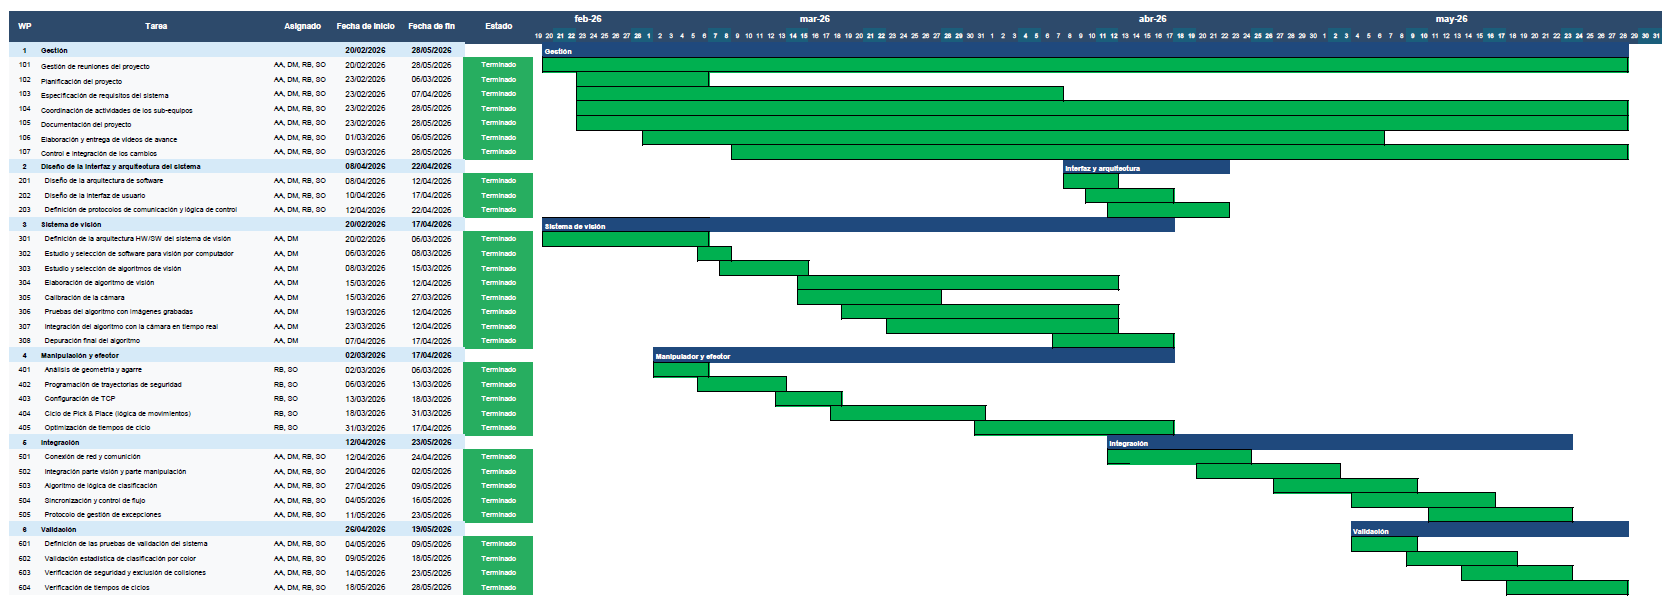
\includegraphics[width=\linewidth]{gantt_definitivo.png}
  \caption{Diagrama de Gantt definitivo del Proyecto REC.}
  \label{fig:gantt}
\end{figure}
\vspace*{\fill}
\end{landscape}

\clearpage
%==============================================================
% 2. DESCRIPCION DEL SISTEMA DESARROLLADO
%==============================================================
\section{Descripción del sistema desarrollado}

El sistema desarrollado clasifica tapones de plástico por color empleando un robot UR3e dotado de un
efector de vacío y un sistema de visión por computador, integrados sobre ROS~2 Humble. La arquitectura
se organiza en cuatro paquetes con responsabilidades separadas: \code{lra\_vision} (infraestructura de
cámara, calibración y modelo cinemático cámara--robot), \code{rec\_vision} (detección y clasificación de
tapones), \code{ur3\_vision\_control} (control del robot y ciclo de pick~\& place) y \code{lra\_hmi}
(interfaz de supervisión y lanzador). En esta sección se describe cada subsistema, sus interfaces y la
algorítmica empleada.

%--------------------------------------------------------------
\subsection{Subsistema de Control}
%--------------------------------------------------------------

\subsubsection{Visión general}

El subsistema de control tiene como objetivo gobernar el robot UR3e para ejecutar ciclos de recogida y
clasificación de tapones de colores sobre una mesa de trabajo. El nodo principal, denominado
\code{ur3\_pick\_sort}, integra la cinemática inversa (IK) mediante MoveIt~2, la gestión de la pinza por
vacío, el control de la visión y la publicación de objetos de colisión en la escena de planificación.

El ciclo de operación completo es el siguiente: el sistema de visión detecta un tapón y publica su
posición en el espacio cartesiano junto con su color; el nodo de control recibe ambos mensajes, resuelve
la trayectoria articular mediante IK, ejecuta las etapas de aproximación, agarre, retirada y depósito en
la caja correspondiente, y finalmente reactiva la visión para el siguiente ciclo.

\subsubsection{Arquitectura software}

\paragraph{Stack tecnológico.}
La Tabla~\ref{tab:ctrl-stack} resume las tecnologías empleadas en el subsistema de control.

\begin{table}[H]
\centering
\caption{Stack tecnológico del subsistema de control.}
\label{tab:ctrl-stack}
\small
\renewcommand{\arraystretch}{1.25}
\begin{tabularx}{\textwidth}{|>{\bfseries}l|>{\RaggedRight\arraybackslash}X|>{\RaggedRight\arraybackslash}X|}
  \hline
  \rowcolor{BlueHeader}
  \textcolor{white}{\bfseries Componente} &
  \textcolor{white}{\bfseries Tecnología / Versión} &
  \textcolor{white}{\bfseries Rol} \\
  \hline
  \rowA Sistema operativo & Ubuntu 22.04 LTS & Plataforma base \\
  \rowB Middleware robótico & ROS 2 Humble & Comunicación inter-proceso \\
  \rowA Planificador de movimiento & MoveIt 2 (Humble) & Planificación de trayectorias e IK \\
  \rowB Controlador de articulaciones & \code{ros2\_control} + \code{scaled\_joint\_trajectory\_controller} & Ejecución de trayectorias en hardware \\
  \rowA Driver del robot & \code{ur\_robot\_driver} & Interfaz con el UR3e real \\
  \rowB Lenguaje de nodos & Python 3.10 & Lógica de control \\
  \rowA Launch system & Python Launch Files (ROS 2) & Orquestación del arranque \\
  \rowB Visualización & RViz 2 (MarkerArray) & Depuración visual en tiempo real \\
  \hline
\end{tabularx}
\end{table}

\paragraph{Nodos ROS 2 del subsistema de control.}
\begin{itemize}
  \item \code{ur3\_pick\_sort} -- Nodo principal. Implementa toda la lógica de pick-and-place, IK, gestión
        de la pinza y coordinación con el sistema de visión (paquete \code{ur3\_vision\_control}).
  \item \code{ur3\_moveit\_test} -- Nodo de prueba de integración con MoveIt~2 a través del \textit{action
        server} \code{/move\_action}. Útil para validar la configuración del stack de forma aislada.
  \item \code{ur3\_simple\_move} (\code{inicio.py}) -- Script de utilidad para llevar el robot a una pose
        articular fija; se usa en la puesta en marcha y la calibración de la posición HOME.
  \item \code{ur3\_controller} (\code{ur3\_controller.py}) -- Prototipo anterior de control directo por
        ángulos heurísticos; no se usa en producción, sirve como referencia de desarrollo.
\end{itemize}

\paragraph{Diagrama de nodos y tópicos.}
La Tabla~\ref{tab:ctrl-topics} describe los tópicos principales con su dirección de flujo respecto al
nodo \code{ur3\_pick\_sort}.

\begin{table}[H]
\centering
\caption{Tópicos y servicios del subsistema de control.}
\label{tab:ctrl-topics}
\scriptsize
\renewcommand{\arraystretch}{1.25}
\begin{tabularx}{\textwidth}{|>{\ttfamily}l|>{\ttfamily}l|c|>{\RaggedRight\arraybackslash}X|}
  \hline
  \rowcolor{BlueHeader}
  \textcolor{white}{\bfseries Tópico} &
  \textcolor{white}{\bfseries Tipo} &
  \textcolor{white}{\bfseries Dir.} &
  \textcolor{white}{\bfseries Descripción} \\
  \hline
  \rowA /ur3/target\_point & geometry\_msgs/Point & Ent. & Posición XYZ del tapón en \code{base\_link} \\
  \rowB /tapones/caja\_asignada & std\_msgs/Int32 & Ent. & Índice de color/caja (1--6) \\
  \rowA /joint\_states & sensor\_msgs/JointState & Ent. & Estado articular (500\,Hz) \\
  \rowB /vision\_enable & std\_msgs/Bool & Sal. & Habilita el detector (latched) \\
  \rowA /scaled\_joint\_traj.../joint\_trajectory & trajectory\_msgs/JointTrajectory & Sal. & Trayectoria al controlador HW \\
  \rowB /io\_and\_status\_controller/set\_io & ur\_msgs/SetIO (srv) & Sal. & Activa/desactiva la ventosa \\
  \rowA /compute\_ik & moveit\_msgs/GetPositionIK (srv) & Bidir. & Solicitud de IK a MoveIt 2 \\
  \rowB /collision\_object & moveit\_msgs/CollisionObject & Sal. & Objetos de colisión (mesa, pared) \\
  \rowA /sorting\_markers & visualization\_msgs/MarkerArray & Sal. & Marcadores RViz (HOME, cajas, target) \\
  \rowB /tf & tf2\_msgs/TFMessage & Ent. & TF \code{base\_link}$\to$\code{tool0} \\
  \hline
\end{tabularx}
\end{table}

\subsubsection{Interfaces entre procesos}

\paragraph{Interfaz con el subsistema de visión.}
La comunicación entre visión y control se realiza exclusivamente mediante tópicos ROS~2, garantizando
desacoplamiento temporal y espacial entre ambos sub-equipos:
\begin{itemize}
  \item \textbf{Posición} (\code{/ur3/target\_point}, \code{geometry\_msgs/Point}): campos $x,y,z$ en
        metros, referenciados a \code{base\_link}. QoS \textit{best-effort}, cola de profundidad~1: el
        controlador procesa únicamente el último \textit{target}, descartando detecciones acumuladas
        durante el ciclo de pick. El nodo de visión publica solo cuando \code{/vision\_enable}=True.
  \vspace{6.5pt}
  \item \textbf{Clasificación} (\code{/tapones/caja\_asignada}, \code{std\_msgs/Int32}): codificación
        1--6 = \{marrón, azul, verde, amarillo y blanco\}. El controlador acepta también cadenas de
        texto vía \code{color\_callback} (nombres en español a índices). Cola de profundidad~1.
  \clearpage      
  \item \textbf{Habilitación} (\code{/vision\_enable}, \code{std\_msgs/Bool}): QoS RELIABLE +
        TRANSIENT\_LOCAL (\textit{latched}). El uso de TRANSIENT\_LOCAL garantiza que cualquier nodo de
        visión que arranque después del controlador reciba inmediatamente el último estado, evitando que
        el detector comience a procesar antes de que el robot haya alcanzado HOME.
\end{itemize}

\paragraph{Interfaz con el hardware del robot (\code{ros2\_control}).}
El UR3e se controla a través del \code{scaled\_joint\_trajectory\_controller}, que escala la velocidad de
ejecución respecto a la máxima configurada en la \textit{teach pendant}. El nodo publica mensajes
\code{JointTrajectory} con un único punto de destino y un tiempo de llegada explícito
(\code{time\_from\_start}); la interpolación la realiza internamente el controlador hardware.

\paragraph{Interfaz con MoveIt 2 (IK).}
La cinemática inversa se resuelve llamando al servicio \code{/compute\_ik}
(\code{moveit\_msgs/GetPositionIK}) de forma asíncrona mediante \code{call\_async()} con un
\code{threading.Event} para el bloqueo, ya que el ciclo de pick-and-place corre en un hilo secundario.
Parámetros relevantes de la petición: \code{group\_name}=\code{ur\_manipulator},
\code{ik\_link\_name}=\code{tool0}, \code{pose\_stamped} en \code{base\_link}, \code{robot\_state}
con semilla articular fija (HOME) para reproducibilidad, \textit{timeout} de 2~s y
\code{avoid\_collisions}=True con \textit{fallback} a False si no se encuentra solución.

\paragraph{Interfaz con la pinza de vacío (\code{SetIO}).}
La ventosa se controla mediante \code{/io\_and\_status\_controller/set\_io} (\code{ur\_msgs/SetIO}):
función=1 (salida digital), pin=4, estado=1.0 (cierre) o 0.0 (apertura). El parámetro
\code{simulate\_gripper} sustituye la llamada real por un \textit{log}, útil para desarrollo sin hardware.


\subsubsection{Interfaz de usuario}

El subsistema de control no dispone de interfaz gráfica propia. La interacción con el operador se realiza
mediante tres mecanismos:
\begin{itemize}
  \item \textbf{Parámetros de lanzamiento} (Tabla~\ref{tab:ctrl-params}), configurables desde el archivo
        de \textit{launch} o la línea de comandos.
  \vspace{6.5pt}
  \item \textbf{Visualización en RViz 2}: el nodo publica un \code{MarkerArray} en \code{/sorting\_markers}
        a 2\,Hz con una esfera blanca (TCP en HOME), cubos de color (las 6 cajas de destino con etiquetas)
        y una esfera magenta (target activo durante el ciclo).
  \vspace{6.5pt}
  \item \textbf{Logs de consola}: el nodo emite logs en cada transición de estado relevante (recepción de
        target, inicio de ciclo, etapas de IK, movimientos, estado de la pinza, tiempos y reactivación de
        visión), permitiendo seguir el sistema sin herramientas externas.
\end{itemize}

\begin{table}[H]
\centering
\caption{Parámetros ROS 2 del nodo \code{ur3\_pick\_sort}.}
\label{tab:ctrl-params}
\small
\renewcommand{\arraystretch}{1.25}
\begin{tabularx}{\textwidth}{|>{\ttfamily}l|l|l|>{\RaggedRight\arraybackslash}X|}
  \hline
  \rowcolor{BlueHeader}
  \textcolor{white}{\bfseries Parámetro} &
  \textcolor{white}{\bfseries Tipo} &
  \textcolor{white}{\bfseries Defecto} &
  \textcolor{white}{\bfseries Descripción} \\
  \hline
  \rowA simulate\_gripper & bool & True & Sustituye la pinza por logs (modo simulación) \\
  \rowB offset\_x & float & 0.0 & Corrección métrica en X del target \\
  \rowA offset\_y & float & 0.0 & Corrección métrica en Y del target \\
  \hline
\end{tabularx}
\end{table}

\paragraph{Scripts de arranque.}
El archivo \code{launch.py} orquesta el arranque completo con temporizaciones explícitas:
$t=0$\,s (MoveIt~2 + cámara + URDF de cámara + calibrador de color), $t=8$\,s (nodo
\code{ur3\_pick\_sort}, tras estabilización de MoveIt) y $t=25$\,s (detector de tapones, tras llegada del
robot a HOME). El archivo \code{launch\_vision.sh} permite arrancar solo el \textit{pipeline} de visión,
útil para calibración y depuración sin el robot activo.

\subsubsection{Algorítmica del sistema de control}

\paragraph{Máquina de estados implícita.}
El nodo implementa una máquina de estados mediante el flag booleano \code{busy} y temporizadores ROS~2
(Tabla~\ref{tab:ctrl-fsm}).

\begin{table}[H]
\centering
\caption{Estados del nodo de control.}
\label{tab:ctrl-fsm}
\scriptsize
\renewcommand{\arraystretch}{1.25}
\begin{tabularx}{\textwidth}{|>{\bfseries}l|>{\RaggedRight\arraybackslash}X|>{\RaggedRight\arraybackslash}X|>{\RaggedRight\arraybackslash}X|}
  \hline
  \rowcolor{BlueHeader}
  \textcolor{white}{\bfseries Estado} &
  \textcolor{white}{\bfseries Entrada} &
  \textcolor{white}{\bfseries Acciones} &
  \textcolor{white}{\bfseries Salida} \\
  \hline
  \rowA INICIALIZANDO & Arranque del nodo & Deshabilita visión, abre pinza, inicia temporizadores de HOME & Robot en HOME \\
  \rowB EN HOME / ESPERANDO & Robot en HOME & Habilita visión, \code{busy}=False & Recepción de target + color \\
  \rowA EJECUTANDO CICLO & \code{try\_start\_cycle()} OK & \code{busy}=True, deshabilita visión, lanza hilo de pick-and-place & Fin de ciclo \\
  \rowB ABORTANDO & Error en IK o movimiento & Retorna a HOME, limpia estado, reactiva visión & Robot en HOME \\
  \hline
\end{tabularx}
\end{table}

\paragraph{Ciclo de pick-and-place.}
El ciclo completo se ejecuta en un hilo secundario (\textit{daemon thread}) para no bloquear el
\textit{executor} de ROS~2, que debe seguir procesando \textit{callbacks} de \code{joint\_states} y
respuestas IK. Las etapas son:
\begin{enumerate}
  \item \textbf{Validación del workspace}: se comprueba que $(x,y,z)$ estén en
        $x\!\in\![-0.60,0.80]$, $y\!\in\![-0.30,0.55]$, $z\!\in\![0.0001,0.30]$~m.
  \item \textbf{IK de APPROACH}: TCP a $\sim$22\,cm sobre el tapón, con semilla fija en HOME.
  \item \textbf{Movimiento bloqueante a APPROACH}: confirmación por \code{/joint\_states} (tol. 0.03\,rad).
  \item \textbf{IK de PICK}: contacto con el tapón (22\,cm $-$ compresión).
  \item \textbf{Movimiento a PICK + cierre de ventosa}: descenso y activación de vacío; espera de 0.7\,s.
  \item \textbf{Movimiento a HOME intermedio}: el robot va directamente a HOME con el tapón.
  \item \textbf{Movimiento a BIN APPROACH}: pose articular pregrabada para el color detectado.
  \item \textbf{Movimiento a BIN DROP}: pose de depósito (pequeña variación angular desde APPROACH).
  \item \textbf{Apertura de ventosa + espera 0.8\,s}: se suelta el tapón.
  \item \textbf{Retorno a BIN APPROACH} (si las poses difieren) y \textbf{HOME final}.
  \item \textbf{Limpieza de estado y reactivación de visión}.
\end{enumerate}

\clearpage
\paragraph{Detección de llegada a waypoint.}
La función \code{move\_to\_joint\_waypoint\_blocking} lee \code{/joint\_states} a 10\,Hz y compara la
posición articular con el objetivo mediante la distancia angular circular:
\begin{equation}
d(a,b)=\bigl|\,((a-b+\pi)\bmod 2\pi)-\pi\,\bigr|.
\end{equation}
El waypoint se considera alcanzado cuando todos los joints cumplen $d<0.03$~rad ($\approx 1.7^\circ$),
con un \textit{timeout} configurable por etapa (entre 8 y 45~s). Si expira, el sistema entra en modo
aborto. Una optimización verifica si el robot ya está en el waypoint antes de publicar la trayectoria,
evitando movimientos redundantes.

\paragraph{Normalización de ángulos.}
Todos los ángulos se normalizan al intervalo $(-\pi,\pi]$ mediante
$\mathrm{normalize}(q)=\operatorname{atan2}(\sin q,\cos q)$. Para evitar giros innecesarios de $360^\circ$
al transitar entre poses se aplica
\begin{equation}
\mathrm{wrap\_to\_near}(q_{\text{ref}},q_{\text{tgt}})
= q_{\text{ref}} + \bigl((q_{\text{tgt}}-q_{\text{ref}}+\pi)\bmod 2\pi - \pi\bigr),
\end{equation}
garantizando que el controlador recibe siempre la solución articular más próxima a la posición actual.


\subsubsection{Matemáticas: cinemática inversa y selección de solución}

\paragraph{Planteamiento.}
Dado un punto objetivo $P=(x,y,z)$ en \code{base\_link}, la IK busca el vector articular
$q=(q_1,\dots,q_6)$ tal que la pose del TCP (\code{tool0}) coincida con la deseada:
$T(q)=T_{\text{base\_link}\to\text{tool0}}(q_1,\dots,q_6)$, donde $T$ es la transformada homogénea
$4\times4$ de la cadena cinemática del UR3e según la convención Denavit--Hartenberg modificada. El solver
es KDL (\textit{Kinematics and Dynamics Library}), integrado en MoveIt~2.

\paragraph{Orientación del TCP.}
Para el pick se requiere el TCP apuntando hacia abajo (perpendicular a la mesa). La orientación base es
una rotación de $\pi$ alrededor de $X$ en el efector, $R_{\text{base}}=\mathrm{Euler}(\pi,0,0)$, es decir
$q=(1,0,0,0)$. Para robustez, se prueban 4 orientaciones variando el \textit{yaw}:
$\{0,+\pi/2,-\pi/2,\pi\}$, ya que la orientación del tapón sobre la mesa es irrelevante para el agarre.

\paragraph{Conversión Euler $\rightarrow$ cuaternión.}
La conversión (ZYX) se implementa directamente, sin dependencias externas, con
$c_\bullet=\cos(\bullet/2)$, $s_\bullet=\sin(\bullet/2)$:
\begin{align}
q_x &= s_r c_p c_y - c_r s_p s_y, &
q_y &= c_r s_p c_y + s_r c_p s_y,\\
q_z &= c_r c_p s_y - s_r s_p c_y, &
q_w &= c_r c_p c_y + s_r s_p s_y.
\end{align}

\paragraph{Búsqueda multi-candidato (\code{solve\_stage\_ik}).}
La función explora un espacio de candidatos para maximizar la probabilidad de hallar una solución IK
válida y de bajo coste (Tabla~\ref{tab:ik-cands}). El espacio total es de hasta
$3\times3\times4\times2=72$ llamadas IK por etapa; en la práctica la primera semilla (HOME) converge en
las primeras iteraciones, por lo que el tiempo real es muy inferior al peor caso.

\begin{table}[H]
\centering
\caption{Dimensiones de búsqueda de \code{solve\_stage\_ik}.}
\label{tab:ik-cands}
\small
\renewcommand{\arraystretch}{1.25}
\begin{tabularx}{\textwidth}{|>{\bfseries}l|c|>{\RaggedRight\arraybackslash}X|}
  \hline
  \rowcolor{BlueHeader}
  \textcolor{white}{\bfseries Dimensión} &
  \textcolor{white}{\bfseries Cand.} &
  \textcolor{white}{\bfseries Descripción} \\
  \hline
  \rowA Semillas articulares & 3 & HOME (fija), posición actual, HOME (respaldo) \\
  \rowB Z del objetivo & 3 & $z_{\text{nom}}$, $z_{\text{nom}}\pm0.02$ (approach) o $\pm0.005$ (pick) \\
  \rowA Orientación TCP (yaw) & 4 & $0,\ +\pi/2,\ -\pi/2,\ \pi$ \\
  \rowB Modo colisión & 2 & \code{avoid\_collisions}=True (primero), False (fallback) \\
  \hline
\end{tabularx}
\end{table}

\paragraph{Función de coste articular.}
Entre todas las soluciones IK válidas se elige la de menor coste, que combina el coste de movimiento y
la penalización por alejarse de la rama preferida de pick:
\begin{align}
\mathrm{coste}(q_{\text{ref}},q_{\text{tgt}}) &= \mathrm{coste}_{\text{mov}} + \mathrm{coste}_{\text{rama}},\\
\mathrm{coste}_{\text{mov}} &= \textstyle\sum_i w_i\, d_{\text{ang}}(q_{\text{ref},i},q_{\text{tgt},i}),\\
\mathrm{coste}_{\text{rama}} &= \lambda \textstyle\sum_i w_i\, d_{\text{ang}}(q_{\text{tgt},i},q_{\text{home},i}),
\end{align}
con pesos $w=[1.0,\,4.0,\,3.5,\,2.0,\,2.0,\,1.0]$ (mayor peso a \textit{shoulder\_lift} y \textit{elbow},
más influyentes en la postura), $\lambda=0.20$ y $d_{\text{ang}}$ la distancia circular mínima entre dos
ángulos. La semilla fija (HOME) garantiza que, ante el mismo target $(x,y)$, el solver devuelve siempre la
misma solución entre arranques.

\paragraph{Geometría TCP y offsets de pick.}
El efector final es un \textit{gripper} neumático más una ventosa, con longitud total de 230\,mm
($L_{\text{gripper}}=137$\,mm, $L_{\text{ventosa}}=93$\,mm). Los offsets Z aplicados a la posición del
tapón se recogen en la Tabla~\ref{tab:offsets}. El offset de compresión de 5\,mm asegura el contacto
firme de la ventosa, necesario para generar el vacío de agarre.

\begin{table}[H]
\centering
\caption{Offsets Z por etapa ($L_{\text{TCP}}=0.230$\,m).}
\label{tab:offsets}
\small
\renewcommand{\arraystretch}{1.25}
\begin{tabularx}{\textwidth}{|>{\bfseries}l|l|>{\RaggedRight\arraybackslash}X|}
  \hline
  \rowcolor{BlueHeader}
  \textcolor{white}{\bfseries Etapa} &
  \textcolor{white}{\bfseries Offset Z (m)} &
  \textcolor{white}{\bfseries Descripción} \\
  \hline
  \rowA APPROACH & $L_{\text{TCP}}+0.08=0.310$ & TCP a 8\,cm sobre el tapón \\
  \rowB PICK (contacto) & $L_{\text{TCP}}-0.005=0.225$ & 5\,mm de compresión \\
  \rowA RETREAT (en HOME) & $L_{\text{TCP}}+0.12=0.350$ & Elevación de seguridad \\
  \hline
\end{tabularx}
\end{table}

\subsubsection{Gestión de la escena de colisión en MoveIt 2}

Para que el solver IK con \code{avoid\_collisions}=True funcione, el nodo publica los objetos de colisión
del entorno físico en \code{/collision\_object} al arrancar (Tabla~\ref{tab:collision}). La mesa está
rotada $45^\circ$ alrededor de $Z$ (cuaternión $[-0.707,0,0,0.707]$) para alinearla con la disposición
física. Estos objetos se eliminan y re-publican en cada arranque para evitar duplicados en la escena
persistente de MoveIt.

\begin{table}[H]
\centering
\caption{Objetos de colisión publicados en la escena.}
\label{tab:collision}
\small
\renewcommand{\arraystretch}{1.25}
\begin{tabularx}{\textwidth}{|>{\ttfamily}l|l|l|>{\RaggedRight\arraybackslash}X|}
  \hline
  \rowcolor{BlueHeader}
  \textcolor{white}{\bfseries Objeto} &
  \textcolor{white}{\bfseries Geom.} &
  \textcolor{white}{\bfseries Posición (world)} &
  \textcolor{white}{\bfseries Dimensiones} \\
  \hline
  \rowA table & BOX & $x{=}0.20,\,y{=}{-}0.10,\,z{=}{-}0.02$ & $1.40\times0.90\times0.04$\,m \\
  \rowB back\_wall & BOX & $x{=}{-}0.25,\,y{=}0.00,\,z{=}0.30$ & $0.06\times0.90\times0.60$\,m \\
  \hline
\end{tabularx}
\end{table}

\subsubsection{Gestión del threading y concurrencia}

El nodo opera con un único \textit{executor} de ROS~2 (\code{rclpy.spin}) en el hilo principal. Para que
los ciclos de pick-and-place (con bucles de espera activa y llamadas bloqueantes) no impidan el
procesamiento de \textit{callbacks}, se separan en un hilo secundario:
\begin{lstlisting}[language=Python]
threading.Thread(target=self.execute_pick_and_place,
                 args=(target, color), daemon=True).start()
\end{lstlisting}
El hilo secundario realiza llamadas asíncronas a los servicios (\code{compute\_ik}, \code{set\_io})
usando \code{threading.Event} para sincronizar y evitar \textit{deadlocks} con el \textit{executor}:
\begin{lstlisting}[language=Python]
future = self.compute_ik_client.call_async(req)
done_event = threading.Event()
future.add_done_callback(lambda fut: done_event.set())
done_event.wait(timeout=timeout_sec + 1.0)
\end{lstlisting}
El flag \code{busy} actúa como \textit{mutex} ligero: solo un ciclo está activo a la vez. Las
suscripciones a \code{/ur3/target\_point} y \code{/tapones/caja\_asignada} retornan inmediatamente si
\code{busy}=True, sin encolar peticiones.

\subsubsection{Configuración de waypoints de destino (bins)}

Las posiciones de depósito de cada color están pregrabadas como vectores articulares en grados,
convertidos a radianes y normalizados al intervalo $(-\pi,\pi]$ en el arranque (Tabla~\ref{tab:bins}).
Para cada color se definen dos waypoints (APPROACH y DROP); la pose de DROP se obtiene aplicando un delta
articular pequeño sobre APPROACH (principalmente \textit{elbow} y \textit{wrist\_1}), produciendo un
descenso hacia el interior de la caja sin recalcular IK. Si APPROACH y DROP son prácticamente iguales
($d<0.03$\,rad en todos los joints), se omite el retorno a APPROACH tras el depósito.

\begin{table}[H]
\centering
\caption{Poses articulares de approach por color/caja (grados).}
\label{tab:bins}
\small
\renewcommand{\arraystretch}{1.25}
\begin{tabularx}{\textwidth}{|>{\bfseries}l|c|>{\RaggedRight\arraybackslash\ttfamily}X|}
  \hline
  \rowcolor{BlueHeader}
  \textcolor{white}{\bfseries Color} &
  \textcolor{white}{\bfseries Caja} &
  \textcolor{white}{\bfseries q (approach)} \\
  \hline
  \rowA Rojo     & 1 & [-252, -108, -68, -96, 87, -60] \\
  \rowB Azul     & 2 & [-236, -114, -56, -99, 90, -50] \\
  \rowA Verde    & 3 & [-223, -139, -14, -118, 90, -35] \\
  \rowB Amarillo & 4 & [-241, -70, -104, -96, 88, -30] \\
  \rowA Negro    & 5 & [-216, -80, -98, -94, 90, -30] \\
  \rowB Blanco   & 6 & [-204, -97, -77, -94, 90, -30] \\
  \hline
\end{tabularx}
\end{table}

\subsubsection{Relación con el subsistema de visión}

El subsistema de control opera de forma completamente reactiva: no realiza procesamiento de imagen ni
decide sobre la identidad o posición de los tapones. Toda esa responsabilidad recae en el subsistema de
visión (Sección~\ref{sec:rec-vision}). La frontera de integración se materializa en tres tópicos ROS~2
que constituyen el contrato de interfaz acordado entre equipos (Tabla~\ref{tab:contrato}).

\begin{table}[H]
\centering
\caption{Contrato de interfaz visión--control.}
\label{tab:contrato}
\scriptsize
\renewcommand{\arraystretch}{1.25}
\begin{tabularx}{\textwidth}{|>{\ttfamily}l|l|l|>{\RaggedRight\arraybackslash}X|}
  \hline
  \rowcolor{BlueHeader}
  \textcolor{white}{\bfseries Tópico} &
  \textcolor{white}{\bfseries Productor} &
  \textcolor{white}{\bfseries Consumidor} &
  \textcolor{white}{\bfseries Semántica} \\
  \hline
  \rowA /vision\_enable & Control & Visión & Indica al detector cuándo puede procesar; False al iniciar cada pick y True al terminar; latched \\
  \rowB /ur3/target\_point & Visión & Control & Posición 3D en \code{base\_link} (m); solo si \code{vision\_enable}=True; cola=1 \\
  \rowA /tapones/caja\_asignada & Visión & Control & Índice de caja (1--6); junto al target; ambos requeridos para iniciar ciclo \\
  \hline
\end{tabularx}
\end{table}

Desde el punto de vista del control, el sistema de visión es una caja negra que produce pares
(posición, color) cuando está habilitado. El único acoplamiento temporal relevante es el arranque: el
nodo \code{ur3\_pick\_sort} publica \code{/vision\_enable}=False al iniciarse y no lo activa hasta que el
robot alcanza físicamente HOME, lo que obliga al detector a permanecer inactivo durante la maniobra
inicial. El \code{launch.py} refleja esta dependencia retrasando el arranque del detector 25\,s respecto
al controlador.

\subsection{Subsistema de Visión}
% =====================================================================
\subsubsection{Infraestructura}
\label{sec:lra-vision}

El paquete \code{lra\_vision} aporta la base sobre la que opera la clasificación: adquisición de imagen,
calibración intrínseca y el modelo cinemático cámara--robot (URDF/TF).

\paragraph{Adquisición de imagen (C++)}
\label{sec:adquisicion}

La captura emplea el nodo \code{v4l2\_camera} lanzado por
\code{camera\_manager.launch.py}, que autodetecta el dispositivo. Los fotogramas se publican como \code{sensor\_msgs/Image}
y los intrínsecos como \code{sensor\_msgs/CameraInfo}. La conversión a matrices OpenCV se realiza con
\code{cv\_bridge}.


\paragraph{Calibración intrínseca}
\label{sec:calib-intrinseca}

El nodo \code{camera\_calibrator\_node} estima los parámetros intrínsecos a partir
de un patrón de ajedrez (método de Zhang). Detecta las esquinas y tras acumular un mínimo de imágenes
ejecuta \code{calibrateCamera}.

\begin{table}[H]
\centering
\caption{Intrínsecos obtenidos (\code{calibration\_data/camera\_info.yaml}, cámara Logitech StreamCam).}
\label{tab:intrinsecos}
\small
\begin{tabular}{@{}llll@{}}
\toprule
$f_x$ & $f_y$ & $c_x$ & $c_y$\\
630.28 & 630.52 & 319.5 & 239.5\\
\midrule
$k_1$ & $k_2$ & $k_3$ & RMS reproyección\\
0.00920 & 0.01708 & $-0.27439$ & 1.111\,px\\
\bottomrule
\end{tabular}
\end{table}

\begin{sloppypar}
El nodo expone un servicio \code{/calibrate\_camera}
(\code{lra\_vision/srv/\penalty0 CalibrateCamera}) con acciones
\code{start}\slash\code{capture}\slash\code{calibrate}\slash\code{save} y publica el progreso en
\code{/camera/calibration/status} (\code{lra\_vision/msg/\penalty0 CalibrationStatus}). La Figura~\ref{fig:calib-flujo} resume el flujo.
\end{sloppypar}

\begin{figure}[H]
\centering
\begin{tikzpicture}[node distance=7mm]
  \node[paso] (cap) {Capturar fotograma\\con patrón};
  \node[decision, below=of cap] (det) {¿esquinas\\detectadas?};
  \node[paso, below=of det] (ref) {\code{cornerSubPix}\\(refino sub-píxel)};
  \node[paso, below=of ref] (acc) {Acumular ($\geq 30$)};
  \node[paso, below=of acc] (calc) {\code{calibrateCamera}\\$\rightarrow K$, distorsión, RMS};
  \node[paso, below=of calc] (save) {Guardar \code{camera\_info.yaml}};
  \draw[flecha] (cap) -- (det);
  \draw[flecha] (det) -- node[lbl]{sí} (ref);
  \draw[flecha] (det.east) -- ++(2.6,0) node[lbl,pos=0.5]{no} |- (cap.east);
  \draw[flecha] (ref) -- (acc);
  \draw[flecha] (acc) -- (calc);
  \draw[flecha] (calc) -- (save);
\end{tikzpicture}
\caption{Flujo de calibración intrínseca.}
\label{fig:calib-flujo}
\end{figure}

\paragraph{Modelo cinemático cámara--robot (URDF/Xacro + TF)}
\label{sec:tf}

La cámara se modela en \code{urdf/camera.xacro} y se monta sobre el efector
\code{tool0} del UR3 mediante uniones fijas, generando los marcos
\code{camera\_link} y \code{camera\_optical\_frame}. El
\code{robot\_state\_publisher} difunde estas transformaciones en \code{/tf}
(Figura~\ref{fig:tf}); son los extrínsecos que \code{rec\_vision}
emplea para pasar de píxel a coordenadas del robot (sección~\ref{sec:pixel3d}).

\begin{figure}[H]
\centering
\begin{tikzpicture}[font=\small]
  \node[blk,    minimum width=20mm] (w) at (0,0)   {\code{world}};
  \node[blk,    minimum width=24mm] (b) at (3.6,0) {\code{base\_link}};
  \node[blk,    minimum width=16mm] (t) at (7.0,0) {\code{tool0}};
  \node[blkcpp, minimum width=30mm, anchor=west] (cl) at (9.4,1.25)  {\code{camera\_link}};
  \node[blkcpp, minimum width=44mm, anchor=west] (co) at (9.4,-1.25) {\code{camera\_optical\_frame}};
  \draw[flecha] (w) -- (b);
  \draw[flecha] (b) -- node[lbl,above,align=center]{cadena\\UR3} (t);
  \draw[flecha] (t.east) -- node[lbl,above,pos=0.5]{fija} (cl.west);
  \draw[flecha] (t.east) -- node[lbl,below,pos=0.5]{fija} (co.west);
\end{tikzpicture}
\caption{Árbol de transformaciones (TF). La cámara cuelga de \code{tool0}.}
\label{fig:tf}
\end{figure}


% =====================================================================
\subsubsection{Clasificación de tapones (\texorpdfstring{\code{rec\_vision}}{rec\_vision})}
\label{sec:rec-vision}

\code{rec\_vision} contiene el núcleo algorítmico. Se organiza en dos nodos coordinados (Figura~\ref{fig:dos-nodos})
y depende de \code{lra\_vision} para los fotogramas, el fichero
\code{camera\_info.yaml} y el TF.

\clearpage
\begin{description}
\item[Nodo 1 --- \code{color\_calibrator\_node}.] Se ejecuta una sola vez
al arrancar: aprende, por aprendizaje no supervisado (K-Means), el color de
referencia de cada caja y lo publica de forma persistente.
\item[Nodo 2 --- \code{vision\_node} / \code{detector\_tapones}.] Se ejecuta en
cada ciclo: detecta los tapones, estabiliza la detección, clasifica el color
comparando con las referencias del Nodo 1, transforma a 3D y publica el objetivo.
\end{description}

\begin{figure}[H]
\centering
\begin{tikzpicture}[node distance=5.5mm]
  % Nodo 1
  \node[paso, fill=recverde!10] (n1a) {Acumular 30 fotogramas\\(detección de tapones)};
  \node[paso, fill=recverde!10, below=of n1a] (n1b) {K-Means en HSV\\($K=$\,\code{num\_cajas})};
  \node[paso, fill=recverde!10, below=of n1b] (n1c) {Publicar \emph{latched}\\\code{centros\_hsv}, \code{num\_cajas}};
  \node[estado, below=of n1c, fill=black!6] (n1d) {Nodo en espera};
  \draw[flecha] (n1a)--(n1b); \draw[flecha](n1b)--(n1c); \draw[flecha](n1c)--(n1d);
  \node[nota, above=1mm of n1a] {\textbf{Nodo 1 (arranque)}};

  % Nodo 2
  \node[paso, right=24mm of n1a, fill=recverde!10] (n2a) {Esperar centros y\\\code{/vision\_enable}$\uparrow$};
  \node[paso, below=of n2a, fill=recverde!10] (n2b) {Muestrear 30 fotogramas};
  \node[paso, below=of n2b, fill=recverde!10] (n2c) {Clustering + clasificación\\de color};
  \node[paso, below=of n2c, fill=recverde!10] (n2d) {Píxel $\rightarrow$ 3D y publicar};
  \draw[flecha](n2a)--(n2b);\draw[flecha](n2b)--(n2c);\draw[flecha](n2c)--(n2d);
  \draw[flechad] (n2d.east) -- ++(1.4,0) node[lbl,pos=0.5]{enable$\downarrow$} |- (n2a.east);
  \node[nota, above=1mm of n2a] {\textbf{Nodo 2 (por ciclo)}};

  \draw[flecha] (n1c.east) to[bend left=10] node[lbl,pos=0.5,align=center]{centros HSV\\(latched)} (n2a.west);
\end{tikzpicture}
\caption{Arquitectura de dos nodos de \code{rec\_vision}.}
\label{fig:dos-nodos}
\end{figure}

\paragraph{Región de interés: detección de la caja}

Para reducir cómputo y descartar detecciones espurias, el procesamiento se limita
a una región de interés (ROI) dinámica: el contorno de mayor área de la
caja de trabajo, segmentada en \textbf{HSV} (más robusto que RGB a cambios de
iluminación)
\begin{equation}
H\in[5,25],\quad S\in[40,255],\quad V\in[40,200]
\end{equation}
Si no se detecta caja, se opera sobre el fotograma completo. Las coordenadas
internas se trasladan después a la imagen global sumando el desplazamiento de la
ROI.

\paragraph{Detección de tapones: transformada de Hough circular}

Dentro de la ROI, la imagen se convierte a escala de grises y se suaviza con un
\textbf{filtro Gaussiano} 9$\times$9 ($\sigma=2$) antes de aplicar
la transformada de Hough, que localiza circunferencias
votando en un espacio de acumulación a partir del gradiente
(Canny interno). Los parámetros se exponen como parámetros
ROS para ajuste en laboratorio.

\paragraph{Extracción robusta de color}
\label{sec:color-robusto}

De cada tapón detectado se extrae un color HSV representativo
con tres salvaguardas: se muestrea un anillo
interior entre $0.25r$ y $0.75r$ (Figura~\ref{fig:anillo}) para evitar el
reflejo especular central y el borde; se descartan píxeles de reflejo o sombra
($V<245 \wedge V>25 \wedge \neg(V>220 \wedge S<40)$), y se agregan los píxeles con
la mediana de $S$ y $V$ (robusta a outliers) y la media
circular del matiz $H$, que es periódico:
\begin{equation}
\theta_i = H_i\cdot\tfrac{2\pi}{180},\qquad
\bar{H} = \left(\operatorname{atan2}\!\Big(\textstyle\frac1N\sum_i\sin\theta_i,\ \frac1N\sum_i\cos\theta_i\Big)\cdot\tfrac{180}{2\pi}\right)\bmod 180.
\label{eq:media-circular}
\end{equation}

\begin{figure}[H]
\centering
\begin{tikzpicture}[scale=1.0]
  \fill[recazul!22, even odd rule] (0,0) circle (1.5) (0,0) circle (0.5);
  \draw[very thick, black!70] (0,0) circle (2);
  \draw[dashed, black!50] (0,0) circle (1.5);
  \draw[dashed, black!50] (0,0) circle (0.5);
  \fill[white] (0,0) circle (0.18);
  \draw (0,0) circle (0.18);
  \node[nota] at (0,-2.45) {borde del tapón ($r$)};
  \node[nota, align=center] at (3.0,0.4) {anillo de muestreo\\$0.25r$ -- $0.75r$};
  \draw[->,>=stealth, black!60] (2.2,0.2) -- (1.0,0.1);
  \node[nota, align=center] at (-2.6,1.3) {reflejo\\central\\(excluido)};
  \draw[->,>=stealth, black!60] (-1.7,1.1) -- (-0.15,0.1);
\end{tikzpicture}
\caption{Máscara anular para la extracción de color.}
\label{fig:anillo}
\end{figure}

\paragraph{Calibración de color por K-Means (Nodo 1)}
\label{sec:kmeans}

El Nodo 1 acumula los colores de unos fotogramas y aplica
\textbf{K-Means} con $K=$\,\code{num\_cajas} sobre el espacio HSV, particionando las
muestras en $K$ grupos que minimizan la inercia intra-clúster:
\begin{equation}
\min_{\{\mu_1,\dots,\mu_K\}}\ \sum_{j=1}^{K}\ \sum_{x\in C_j}\ \lVert x-\mu_j\rVert^2 .
\label{eq:kmeans}
\end{equation}
Los centroides $\mu_j=(H_j,S_j,V_j)$ son el \textbf{color de referencia} de cada
caja. Este enfoque
no supervisado evita umbrales de color codificados: el sistema se adapta a
los tapones reales presentes. Los centroides y el número de cajas se publican para que el Nodo 2 los reciba. El parámetro \code{num\_cajas} es configurable.

\begin{figure}[H]
\centering
\begin{tikzpicture}
\begin{axis}[width=0.74\linewidth, height=5.2cm,
    xlabel={Matiz $H$ (0--180)}, ylabel={Saturación $S$ (0--255)},
    xmin=0,xmax=180, ymin=80, ymax=255, grid=both, grid style={black!10},
    title={\small Centroides HSV aprendidos por K-Means (ilustrativo)},
    legend style={font=\scriptsize, at={(1.02,1)}, anchor=north west}]
  \addplot[only marks, mark=*, mark size=1pt, recnaranja!70] coordinates {
    (4,205)(6,212)(3,198)(7,220)(5,190)(8,208)};
  \addplot[only marks, mark=*, mark size=1pt, color=olive] coordinates {
    (27,200)(29,210)(26,195)(30,205)(28,188)};
  \addplot[only marks, mark=*, mark size=1pt, recverde!70] coordinates {
    (60,172)(58,165)(62,180)(59,158)(61,170)};
  \addplot[only marks, mark=*, mark size=1pt, recazul!70] coordinates {
    (110,190)(112,182)(108,198)(111,176)(109,188)};
  \addplot[only marks, mark=star, mark size=4pt, black] coordinates {
    (5,205)(28,199)(60,169)(110,187)};
  \legend{rojo, amarillo, verde, azul, centroides}
\end{axis}
\end{tikzpicture}
\caption{Muestras de color y centroides ($\mu_j$) de cada caja en el plano matiz--saturación.}
\label{fig:hsv-clusters}
\end{figure}

\paragraph{Clasificación por color (Nodo 2)}
\label{sec:clasificacion}

El color del tapón objetivo se compara con cada centroide mediante una
\textbf{distancia HSV ponderada} que respeta la
circularidad del matiz y atenúa $H$ cuando la saturación es baja.
La caja asignada es la del centroide más cercano:
$\text{caja}=\arg\min_{j} d(c_{\text{tapón}},\mu_j)+1$.

\clearpage
\paragraph{Estabilidad temporal multifotograma}

La detección fotograma a fotograma es ruidosa. Para enviar al robot un objetivo
\textbf{estable}, el Nodo 2 acumula 30 fotogramas y agrupa todas las detecciones
en clústeres espaciales (umbral de 10\,px entre centros). El clúster
ganador es el de mayor número de apariciones (el tapón cuya posición ha
sido más consistente en el tiempo). Su posición se promedia y su color se resume
con media circular de $H$ y mediana de $S,V$ (sección~\ref{sec:color-robusto}) antes de
clasificar.

\paragraph{Transformación píxel \texorpdfstring{$\rightarrow$}{->} 3D}
\label{sec:pixel3d}

Conocido el píxel $(\bar u,\bar v)$ del objetivo, se obtiene su posición 3D en el
marco \code{base\_link} (Figura~\ref{fig:rayo}). Primero se corrige la distorsión y
se obtiene el rayo de proyección en el marco óptico. Con la rotación $R$ y
traslación $T$ de \code{camera\_optical\_frame} a \code{base\_link}, el rayo en el
marco del robot es $\mathbf{r}_{\text{base}}=R\,\mathbf{r}_{\text{cam}}$, y su
intersección con el plano $z=z_t$ de la mesa da la posición del tapón.

\begin{figure}[H]
\centering
\begin{tikzpicture}[scale=0.95]
  \draw[fill=black!5] (-0.5,0) -- (5.5,0) -- (6.5,1) -- (0.5,1) -- cycle;
  \node[nota] at (5.6,0.35) {plano $z=z_t$};
  \fill (1.2,3.4) circle (2pt) node[above,nota]{cámara $C$ ($T$)};
  \fill (4.0,0.55) circle (2pt) node[below right,nota]{$\mathbf{P}$};
  \draw[flecha] (1.2,3.4) -- (4.0,0.55);
  \node[nota] at (3.0,2.3) {$\mathbf{r}_{\text{base}}$};
  \draw[<->,>=stealth, black!55] (1.2,3.4) -- (1.2,0.62);
  \node[nota,rotate=90] at (0.95,2.0) {$\Delta Z=T_z-z_t$};
  \draw[->,black!70] (0.2,0.2) -- (1.1,0.2) node[right,nota]{$x$};
  \draw[->,black!70] (0.2,0.2) -- (0.2,1.0) node[above,nota]{$z$};
  \node[nota] at (0.2,0.0) {\code{base\_link}};
\end{tikzpicture}
\caption{Geometría de la intersección rayo--plano para recuperar la profundidad.}
\label{fig:rayo}
\end{figure}

\paragraph{Interbloqueo visión--robot}
\label{sec:interlock}

La sincronización entre visión y manipulación se resuelve con un
interbloqueo sobre el tópico \code{/vision\_enable}. El detector arranca deshabilitado, cada flanco de
subida reinicia el muestreo y produce una única detección nueva, y el
flanco de bajada detiene la publicación mientras el robot maniobra
(Figura~\ref{fig:interlock}). Así se evita enviar objetivos contradictorios
durante el pick \& place. La parada de emergencia de la HMI fuerza este
tópico a \code{False}.

\begin{figure}[H]
\centering
\begin{tikzpicture}[node distance=0mm]
  \node[blkext] (R) at (0,0) {\code{ur3\_pick\_sort} (robot)};
  \node[blkpy] (V) at (7,0) {\code{detector\_tapones} (visión)};
  \draw[thick,black!40,dashed] (R.south) -- ++(0,-5.2);
  \draw[thick,black!40,dashed] (V.south) -- ++(0,-5.2);
  \draw[flecha] (0,-0.8) -- node[lbl,pos=0.5]{\code{/vision\_enable}=True ($\uparrow$)} (7,-0.8);
  \node[draw,fill=recverde!10,font=\scriptsize,align=center,minimum width=22mm] at (7,-1.6) {muestreo 30 fot.\\+ clasificación};
  \draw[flecha] (7,-2.3) -- node[lbl,pos=0.5,align=center]{\code{target\_point}\\+\,\code{caja\_asignada}} (0,-2.3);
  \node[draw,fill=black!6,font=\scriptsize,align=center,minimum width=22mm] at (0,-3.1) {pick \& place};
  \draw[flecha] (0,-3.8) -- node[lbl,pos=0.5]{\code{/vision\_enable}=False ($\downarrow$)} (7,-3.8);
  \node[nota] at (3.5,-4.6) {(se repite en el siguiente ciclo)};
\end{tikzpicture}
\caption{Diagrama de secuencia del interbloqueo visión--robot.}
\label{fig:interlock}
\end{figure}

\clearpage
% =====================================================================
\subsection{Interfaz Hombre-Máquina}
\label{sec:hmi}

\code{lra\_hmi} es una interfaz de
supervisión de estilo \textbf{SCADA} que actúa como centro de mando del
sistema: lanza y vigila todos los subsistemas, muestra telemetría y permite la
parada de emergencia.

\subsubsection{Arquitectura}

La HMI se estructura en una ventana y tres componentes desacoplados
(Figura~\ref{fig:hmi-arq}):
\begin{itemize}
\item \code{RosBridge}: nodo que traduce suscripciones ROS en señales
para la HMI.
\item \code{ProcessManager}: lanza/para/reinicia cada subsistema como
subproceso en su propio grupo de procesos.
\item \code{ConnectionMonitor}: hilo que hace \emph{ping} periódico al robot.
\end{itemize}

\begin{figure}[H]
\centering
\begin{tikzpicture}[node distance=6mm and 12mm]
  \node[blkhmi, minimum width=42mm] (mw) {\code{MainWindow}\\\scriptsize 5 pestañas (panel, cámara, registros, ajustes, acerca de)};
  \node[blk, below left=12mm and 2mm of mw] (rb) {\code{RosBridge}\\\scriptsize (rclpy)};
  \node[blk, below=12mm of mw] (pm) {\code{ProcessManager}};
  \node[blk, below right=12mm and 2mm of mw] (cm) {\code{ConnectionMonitor}};
  \node[blkext, below=8mm of rb] (ros) {Tópicos ROS\,2};
  \node[blkext, below=8mm of pm] (subp) {Subprocesos\\\scriptsize \code{ros2 launch/run}};
  \node[blkext, below=8mm of cm] (rob) {UR3 (ping)};
  \draw[flecha] (mw) -- (rb); \draw[flecha] (mw) -- (pm); \draw[flecha] (mw) -- (cm);
  \draw[{Latex}-{Latex}] (rb) -- (ros);
  \draw[flecha] (pm) -- (subp);
  \draw[flecha] (cm) -- (rob);
\end{tikzpicture}
\caption{Componentes de la HMI.}
\label{fig:hmi-arq}
\end{figure}

\subsubsection{Disposición de la interfaz}

\begin{figure}[H]
\centering
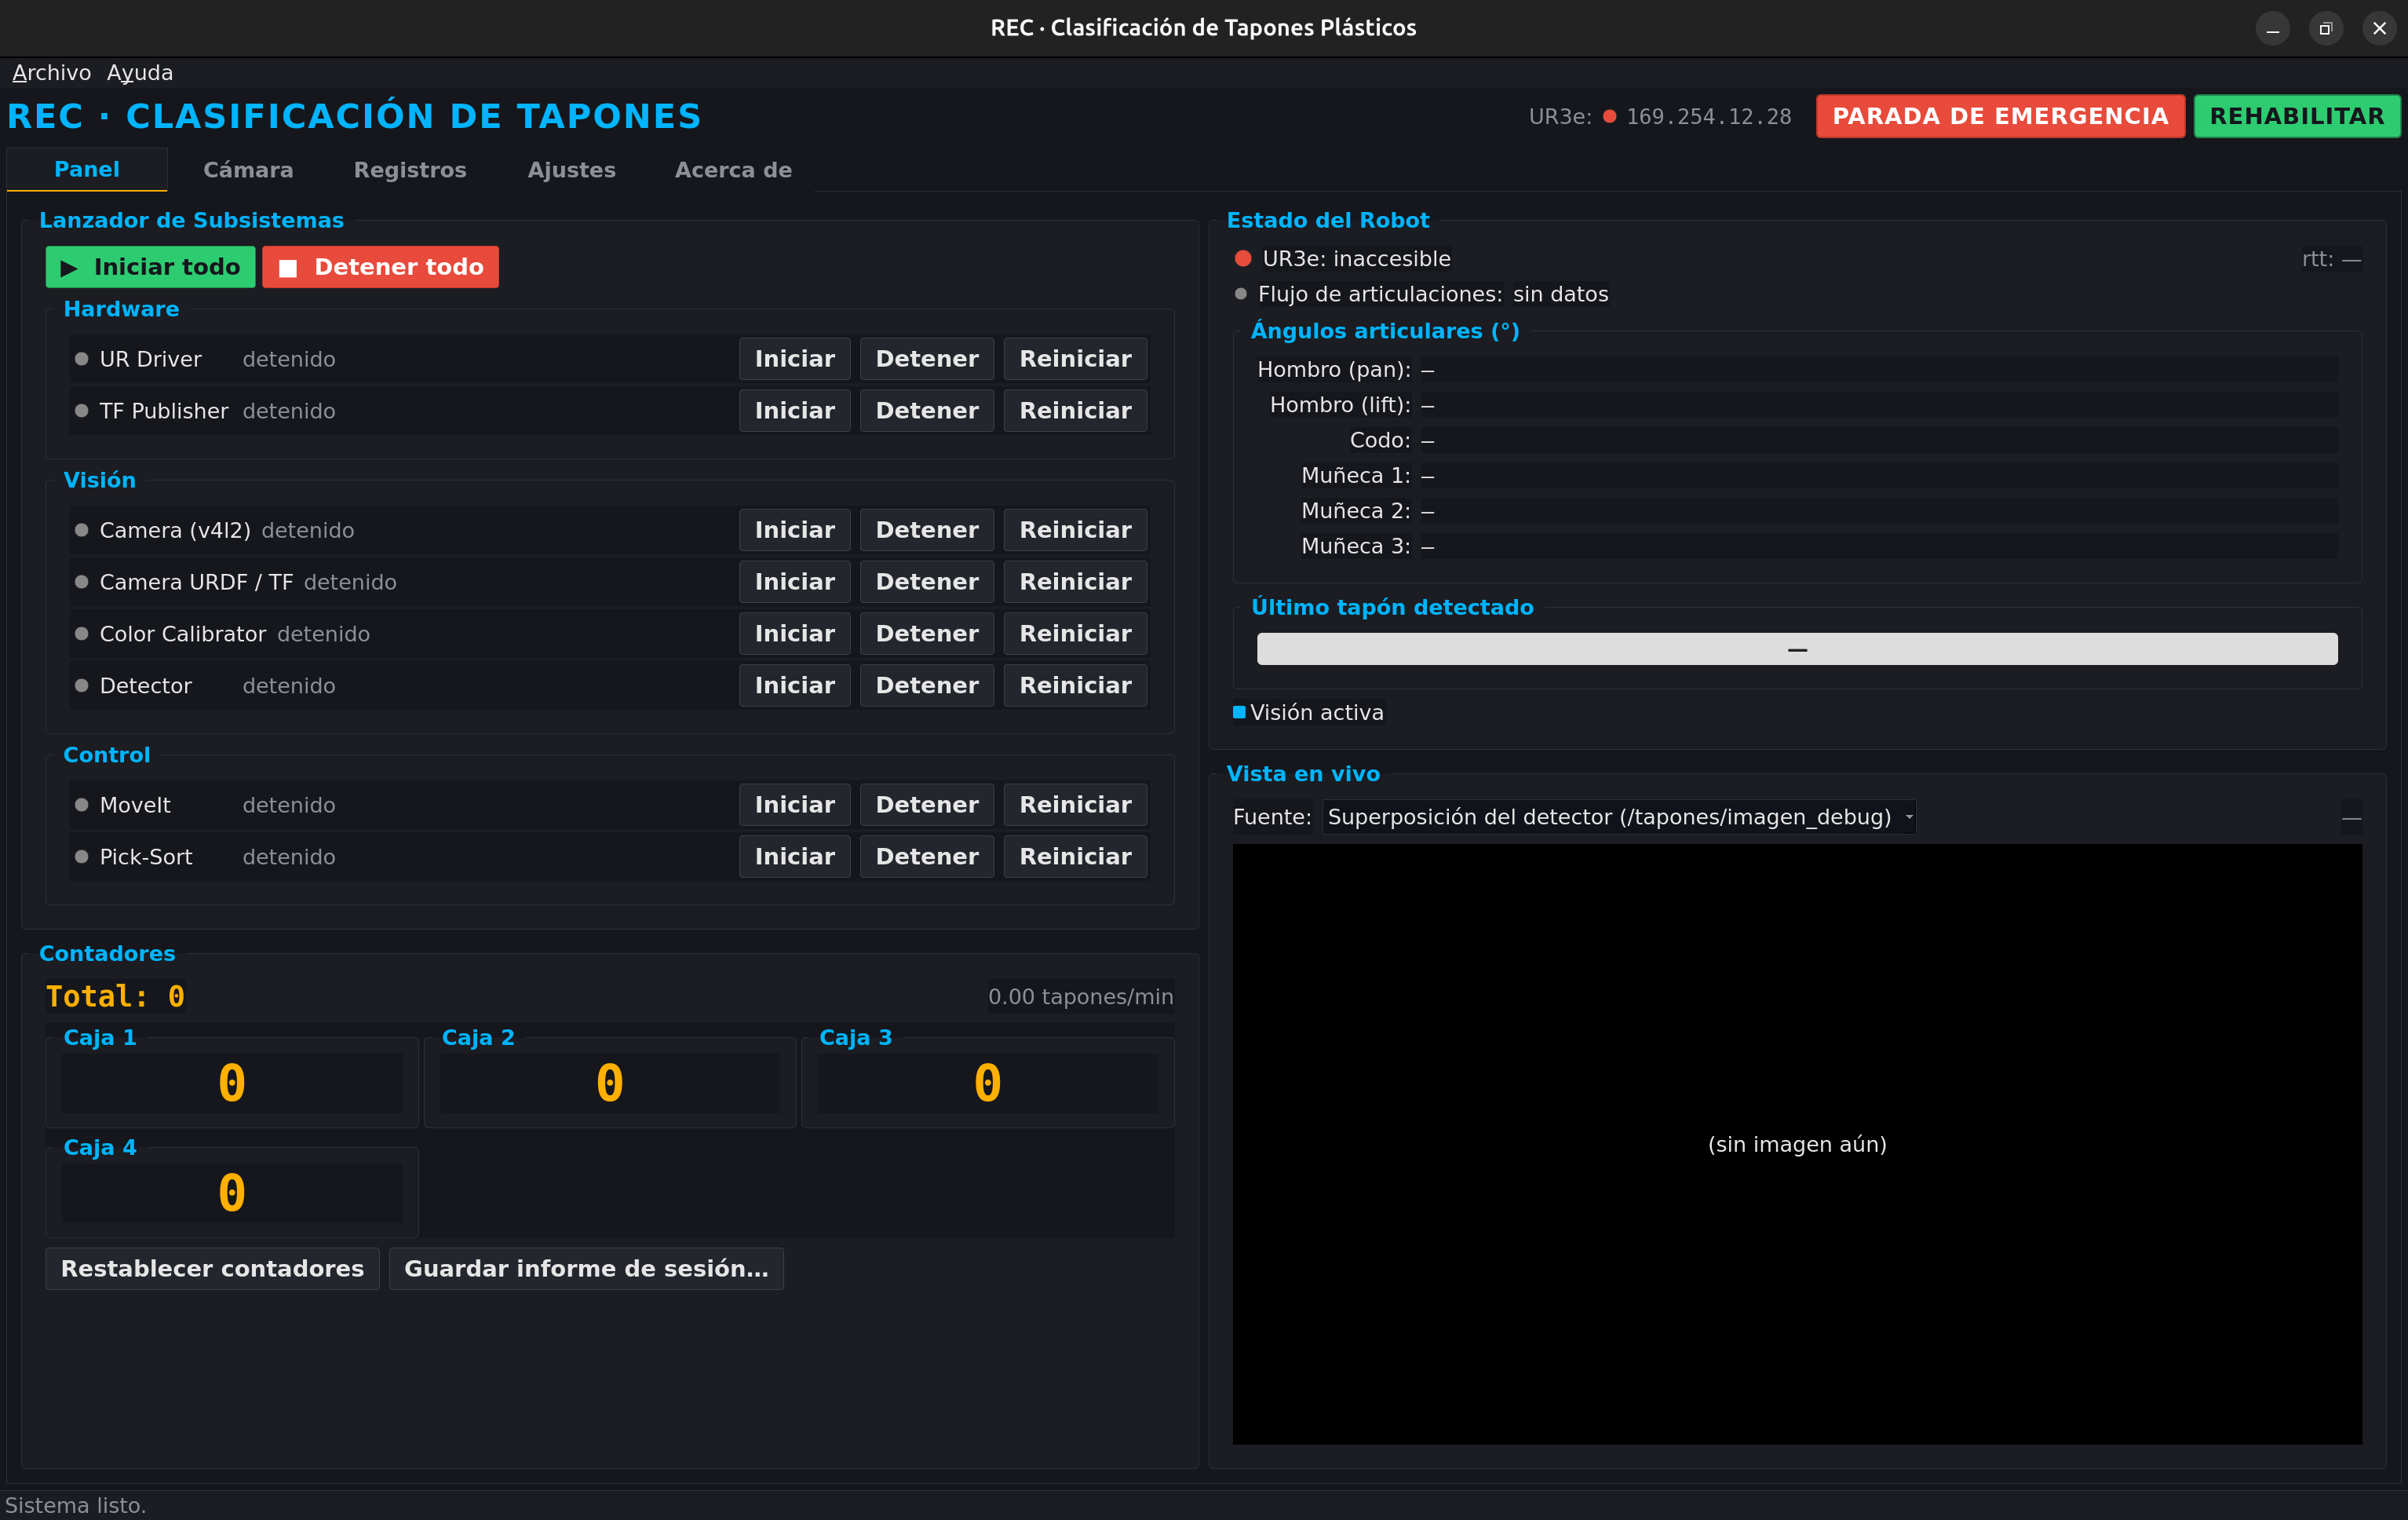
\includegraphics[width=\linewidth]{Screenshot from 2026-05-29 00-30-25.png}
\caption{Captura de la HMI.}
\label{fig:hmi-foto}
\end{figure}

La ventana (Figura~\ref{fig:hmi-foto}) tiene una barra superior siempre
visible (título, LED de conexión del UR3e, IP, botón \textbf{PARADA DE
EMERGENCIA} y \textbf{REHABILITAR}) y cinco pestañas. La pestaña Panel
agrupa lanzador, contadores, estado y vista de cámara.

\subsubsection{Gestión de procesos}

\code{ProcessManager} lanza cada subsistema (Tabla~\ref{tab:subsistemas}), creando un grupo de procesos
propio que permite detenerlo limpiamente
o de forma inmediata (E-stop). Cada subsistema sigue la máquina de estados de la
Figura~\ref{fig:fsm}.

\begin{figure}[H]
\centering
\begin{tikzpicture}[node distance=14mm and 22mm]
  \node[estado] (st) {STOPPED};
  \node[estado, right=of st] (sa) {STARTING};
  \node[estado, right=of sa] (ru) {RUNNING};
  \node[estado, below=of sa] (cr) {CRASHED};
  \node[estado, below=of ru] (so) {STOPPING};
  \draw[flecha] (st) -- node[lbl]{iniciar} (sa);
  \draw[flecha] (sa) -- node[lbl]{ok} (ru);
  \draw[flecha] (sa) -- node[lbl]{fallo} (cr);
  \draw[flecha] (ru) -- node[lbl]{detener} (so);
  \draw[flecha] (ru) -- node[lbl]{exit$\neq$0} (cr);
  \draw[flecha] (so) -- node[lbl,pos=0.4]{fin} (st);
  \draw[flecha] (cr) -- node[lbl]{reiniciar} (st);
\end{tikzpicture}
\caption{Máquina de estados por subsistema (\code{ProcessManager}).}
\label{fig:fsm}
\end{figure}

\begin{table}[H]
\centering
\caption{Subsistemas gestionados por la HMI.}
\label{tab:subsistemas}
\small
\begin{tabular}{l l}
\toprule
\textbf{Clave} & \textbf{Sección}\\
\midrule
driver & Hardware\\
tf & Hardware\\
moveit & Control\\
camera & Visión\\
camera\_urdf & Visión\\
calibrator & Visión\\
detector & Visión\\
pick\_sort & Control\\
\bottomrule
\end{tabular}
\end{table}

\subsubsection{Supervisión, seguridad y configuración}

\begin{itemize}
\item \textbf{Telemetría.} La HMI incrementa el contador de la caja recibida, muestra el total, y permite exportar un
informe JSON de la sesión (duración, total y conteo por caja). Presenta
los ángulos articulares y el color del último tapón.
\item \textbf{Seguridad.} \textbf{PARADA DE EMERGENCIA} mata todos los
subprocesos, \textbf{REHABILITAR}
reactiva la visión. El \code{ConnectionMonitor} señala la pérdida de conexión con
el robot.
\item \textbf{Configuración.} La pestaña Ajustes edita los
parámetros de cada subsistema (cámara, calibrador, detector, pick \& sort) y
los persiste en un archivo de configuración, fusionados sobre los
valores por defecto del paquete; al cambiar parámetros que afectan a un subsistema
en ejecución, avisa de que debe reiniciarse.
\end{itemize}

% =====================================================================
\clearpage
\subsection{Entorno de construcción y despliegue (Docker / ROS\,2 Humble)}
\label{sec:docker}

Todo el workspace se compila y ejecuta dentro de un contenedor
\textbf{Docker} basado en \code{ros:humble} (Figura~\ref{fig:docker}). Esta
decisión aporta reproducibilidad (dependencias fijadas en el
\code{Dockerfile}).

\begin{figure}[H]
\centering
\begin{tikzpicture}[node distance=6mm and 14mm]
  \node[draw, very thick, rounded corners, fill=black!4, minimum width=62mm, minimum height=34mm] (host) {};
  \node[anchor=north west, nota] at (host.north west) {\ \ Host};
  \node[draw, very thick, rounded corners, fill=recazul!10, minimum width=46mm, minimum height=22mm] (cont) at ($(host.center)+(0,-0.2)$) {};
  \node[anchor=north west, nota] at (cont.north west) {\ Contenedor \code{ros:humble}};
  \node[blkpy] (ws) at (cont.center) {\emph{workspace} \code{lra\_ws}\\\scriptsize (lra\_vision, rec\_vision, lra\_hmi)};
  \node[blkext, right=18mm of host, yshift=8mm] (ur) {UR3\\\scriptsize 169.254.x.x};
  \node[blkext, right=18mm of host, yshift=-10mm] (usb) {Cámara USB};
  \node[blkext, below=8mm of host] (x11) {X11 (\code{DISPLAY})};
  \draw[{Latex}-{Latex}] (cont.east) -- node[lbl,pos=0.5]{red host} (ur.west);
  \draw[flecha] (usb.west) -- node[lbl,pos=0.5]{privileged} (cont.east);
  \draw[{Latex}-{Latex}] (cont.south) -- node[lbl,pos=0.5]{socket X11} (x11.north);
\end{tikzpicture}
\caption{Despliegue en contenedor: aislamiento sobre el host, con red \emph{host}, cámara USB y GUI por X11.}
\label{fig:docker}
\end{figure}


\clearpage
%==============================================================
% 3. PRUEBAS DE VALIDACION
%==============================================================
\section{Pruebas de validación}

%--------------------------------------------------------------
\subsection{Definición de las pruebas}
%--------------------------------------------------------------

Para verificar el correcto funcionamiento de la integración de las partes de visión y manipulación, se
definieron cuatro pruebas englobadas en el paquete de trabajo WP-600 (Validación):

\begin{enumerate}
  \item \textbf{Prueba 601: Definición de las pruebas de validación del sistema.}
        \textit{Objetivo:} establecer el protocolo, el entorno físico y digital, y los criterios de
        aceptación para el resto de las pruebas.
  \item \textbf{Prueba 602: Validación estadística de clasificación por color.}
        \textit{Objetivo:} verificar la robustez del algoritmo de segmentación y clasificación cromática
        de los tapones bajo condiciones de ciclo continuo (detección y agarre).
  \item \textbf{Prueba 603: Verificación de seguridad y exclusión de colisiones.}
        \textit{Objetivo:} garantizar que el planificador de trayectorias (\code{MoveIt}) descarte rutas
        que comprometan la integridad del robot, detecte obstáculos virtuales y gestione correctamente
        los límites del espacio de trabajo.
  \item \textbf{Prueba 604: Verificación de tiempos de ciclos.}
        \textit{Objetivo:} medir los tiempos finales de ejecución del proceso optimizado (detección,
        aproximación, agarre, transporte y depósito) para comprobar si cumplen las especificaciones.
\end{enumerate}

%--------------------------------------------------------------
\subsection{Desarrollo de las pruebas y resultados}
%--------------------------------------------------------------

\subsubsection{Prueba 602: Clasificación por color en ciclo continuo}

\textbf{Procedimiento.} Para comprobar la correcta clasificación por color del sistema de visión, se
introdujeron en la caja 20 tapones de diferentes colores (distintos tonos de azul, verde y amarillo,
además de blanco, marrón y rojos) y se predefinieron 6 cajas de clasificación. El sistema debía calibrar
por color los tapones presentes, dividirlos en 6 grupos y clasificarlos en las cajas. La prueba se
ejecutó un total de 20 veces.

\textbf{Resultados.} El sistema clasificó correctamente 18 de 20 tapones, lo que da una tasa de acierto
del 90\,\% respecto al color. Los dos tapones restantes sí fueron depositados en otras cajas sin generar
error, por lo que se obtuvo un 100\,\% de aciertos respecto al posicionamiento. No se observaron errores
de desviación en el agarre de los tapones ni en las trayectorias.

\subsubsection{Prueba 603: Seguridad y exclusión de colisiones}

\textbf{Procedimiento.} Se realizaron tres pruebas en el entorno controlado de \code{MoveIt} y en el
entorno físico:
\begin{enumerate}
  \item \textit{Invasión de obstáculos:} para comprobar que el sistema es capaz de detectar y esquivar
        obstáculos, se generó un obstáculo virtual en la trayectoria hacia una de las cajas.
  \item \textit{Coordenada prohibida:} se envió directamente una coordenada por detrás de la pared
        trasera.
  \clearpage      
  \item \textit{Retorno seguro:} se forzó una parada en mitad del ciclo y, desde ese punto, se probó la
        vuelta a la posición de HOME para verificar que el robot no invade ninguna zona restringida.
\end{enumerate}

\textbf{Resultados.}
\begin{enumerate}
  \item El planificador recalculó trayectorias alternativas esquivando el obstáculo virtual añadido.
  \item Al enviar la coordenada por detrás de la pared, \code{MoveIt} bloqueó la ejecución del movimiento
        devolviendo el error esperado de trayectoria inalcanzable, impidiendo que el UR3 colisionara.
  \item El retorno a HOME se realizó a través de un espacio seguro, sin invadir las zonas de los
        contenedores.
\end{enumerate}

\subsubsection{Prueba 604: Verificación de tiempos de ciclos}

\textbf{Procedimiento.} Tras aumentar la velocidad del robot, se cronometraron 5 ciclos completos. Los
tiempos por ciclo se muestran en la Tabla~\ref{tab:tiempos}.

\begin{table}[H]
\centering
\caption{Tiempos de ciclo registrados tras la optimización del sistema.}
\label{tab:tiempos}
\small
\renewcommand{\arraystretch}{1.25}
\begin{tabularx}{\textwidth}{|>{\bfseries}l|
    >{\centering\arraybackslash}X|
    >{\centering\arraybackslash}X|
    >{\centering\arraybackslash}X|
    >{\centering\arraybackslash}X|}
  \hline
  \rowcolor{BlueHeader}
  \textcolor{white}{\bfseries ID Ciclo} &
  \textcolor{white}{\bfseries Detección Visión (s)} &
  \textcolor{white}{\bfseries Trayectoria y Agarre (s)} &
  \textcolor{white}{\bfseries Transporte y Depósito (s)} &
  \textcolor{white}{\bfseries Tiempo Total (s)} \\
  \hline
  \rowA Ciclo 1 & $<2$ & 10 & 27 & \textbf{39} \\
  \rowB Ciclo 2 & $<2$ & 11 & 26 & \textbf{39} \\
  \rowA Ciclo 3 & $<2$ & 10 & 31 & \textbf{43} \\
  \rowB Ciclo 4 & $<2$ & 12 & 27 & \textbf{41} \\
  \rowA Ciclo 5 & $<2$ & 11 & 30 & \textbf{43} \\
  \hline
  \rowcolor{BlueCell}
  \textbf{Media} & $<2$ & \textbf{10.8} & \textbf{28.2} & \textbf{41} \\
  \hline
\end{tabularx}
\end{table}

%--------------------------------------------------------------
\subsection{Análisis de resultados y validación de objetivos (requisitos)}
%--------------------------------------------------------------

Una vez comprobadas las pruebas de validación del paquete WP-600, se comparan los resultados obtenidos
con los requisitos iniciales del proyecto:

\begin{enumerate}
  \item \textbf{Precisión y clasificación (robustez).} La prueba 602 valida que la integración de la
        cámara y el software de visión es capaz de extraer las coordenadas precisas de los tapones y
        asociarlos a un filtro de color correcto. Con un 90\,\% de aciertos en color, se considera un
        porcentaje suficientemente alto para asumir un funcionamiento correcto y fiable ante variaciones
        de la posición de los tapones (con un 100\,\% de aciertos en posicionamiento).
  \item \textbf{Seguridad (integridad).} Los resultados de la prueba 603 confirman que las herramientas
        empleadas (\code{MoveIt} / ROS) eliminan por completo el riesgo de colisión física, tanto por
        fallos de programación como por introducción de coordenadas erróneas. El robot mantiene un
        comportamiento seguro, respetando los límites cinemáticos, geométricos y del entorno real.
  \clearpage
  \item \textbf{Eficiencia temporal (rendimiento).} El análisis de la prueba 604 muestra un tiempo medio
        por ciclo de \textbf{41~segundos}. Este valor, aunque adecuado, no corresponde a una gran
        optimización del tiempo de ciclo.
\end{enumerate}

\noindent\textbf{Conclusión de la validación.}
Se han cumplido satisfactoriamente todos los criterios de aceptación de las pruebas del paquete WP-600.
Por tanto, se alcanza con éxito el hito \textbf{H7 (Validación del sistema)} y queda confirmada la
aceptación final del proyecto, con el sistema listo para el hito \textbf{H8 (Sistema final operativo)} y
su demostración.

\clearpage
%==============================================================
% 4-8. SECCIONES PENDIENTES
%==============================================================
\section{Lista de materiales}

\begin{table}[H]
\centering
\caption{Lista de materiales del sistema.}
\label{tab:bom}
\small
\renewcommand{\arraystretch}{1.3}
\begin{tabularx}{\textwidth}{|c|>{\RaggedRight\arraybackslash}X|c|>{\RaggedRight\arraybackslash}X|}
  \hline
  \rowcolor{BlueHeader}
  \textcolor{white}{\bfseries \#} &
  \textcolor{white}{\bfseries Componente} &
  \textcolor{white}{\bfseries Ud.} &
  \textcolor{white}{\bfseries Observaciones} \\
  \hline
  \multicolumn{4}{|l|}{\cellcolor{BlueCell}\bfseries Hardware robótico} \\
  \hline
  \rowA 1 & Robot colaborativo Universal Robots UR3e & 1 & 6 GDL, alcance 500\,mm, carga útil 3\,kg \\
  \rowB 2 & Controlador del UR3e (CB-Series) & 1 & Incluido con el robot; conexión Ethernet \\
  \rowA 3 & Teach Pendant del UR3e & 1 & Pantalla táctil para configuración y modo manual \\
  \hline
  \multicolumn{4}{|l|}{\cellcolor{BlueCell}\bfseries Efector final} \\
  \hline
  \rowB 4 & Soporte de gripper neumático & 1 & Montado sobre \code{tool0} \\
  \rowA 5 & Ventosa de vacío & 1 & Acoplada al gripper. Control por salida digital (pin 4) \\
  \hline
  \multicolumn{4}{|l|}{\cellcolor{BlueCell}\bfseries Sistema de visión} \\
  \hline
  \rowB 6 & Cámara Logitech StreamCam & 1 &  \\
  \rowA 7 & Soporte de cámara sobre el efector & 1 & Fijación sobre \code{tool0} (definido en URDF/Xacro) \\
  \hline
  \multicolumn{4}{|l|}{\cellcolor{BlueCell}\bfseries Entorno de trabajo} \\
  \hline
  \rowB 8 & Mesa de trabajo & 1 & Superficie del laboratorio  \\
  \rowA 9 & Caja de trabajo (zona de recogida) & 1 & Caja rectangular donde se depositan los tapones a clasificar \\
  \rowB 10 & Cajas de clasificación (destino) & 6 & Número configurable desde la HMI \\
  \rowA 11 & Tapones de plástico de colores  & $\sim$15 & Azul, verde, amarillo, blanco, marrón \\
  \hline
  \multicolumn{4}{|l|}{\cellcolor{BlueCell}\bfseries Computación y red} \\
  \hline
  \rowB 12 & PC de desarrollo y ejecución & 1 & Ubuntu 22.04 con ROS\,2 Humble \\
  \rowA 13 & Cable Ethernet (PC $\leftrightarrow$ UR3e) & 1 & Conexión directa, red 169.254.x.x \\
  \rowB 14 & Cable USB (PC $\leftrightarrow$ cámara) & 1 & USB Type-C \\
  \hline
  \multicolumn{4}{|l|}{\cellcolor{BlueCell}\bfseries Software (desarrollo propio)} \\
  \hline
  \rowA 15 & lra\_vision & -- & Adquisición de imagen, calibración intrínseca, URDF cámara \\
  \rowB 16 & rec\_vision & -- & Detección y clasificación de tapones (K-Means, Hough, TF2) \\
  \rowA 17 & ur3\_vision\_control & -- & Control del UR3e, ciclo pick\,\&\,place, IK vía MoveIt\,2 \\
  \rowB 18 & lra\_hmi & -- & Interfaz de supervisión PyQt5 (HMI tipo SCADA) \\
  \hline
\end{tabularx}
\end{table}

\clearpage
La Tabla~\ref{tab:bom} recoge los componentes principales del sistema desarrollado.
Los elementos de hardware robótico y el entorno de trabajo fueron proporcionados por
el Laboratorio de Automática y Robótica (LAR) de la UPM. El software es íntegramente
de desarrollo propio sobre herramientas de código abierto.

Todos los componentes de hardware fueron proporcionados por el laboratorio. El coste del
proyecto es exclusivamente de horas de ingeniería.

\section{Vídeos}
\textit{[ Pendiente: incluir enlaces a los vídeos de seguimiento y demostración final. ]}

\section{ANEXO I: Especificación de Requisitos}

\subsection{Requisitos Funcionales y de Operación}

\begin{itemize}
    \item \textbf{RF-01. Clasificación de tapones:} El sistema deberá detectar, identificar y clasificar tapones plásticos en un número parametrizable de categorías (por defecto 4, ampliable hasta 6), de acuerdo con la calibración dinámica de color implementada.
    \item \textbf{RF-02. Conteo de elementos clasificados:} El sistema deberá visualizar el número de tapones clasificados por cada categoría, así como el total acumulado y la tasa de procesamiento (tapones/minuto). Además, se permitirá la exportación de un informe de sesión en formato JSON.
    \item \textbf{RF-03. Control de operación por el usuario:} El usuario gestionará el ciclo de vida de los subsistemas (iniciar, detener, reiniciar) a través de una Interfaz Hombre-Máquina (HMI). La interfaz incluirá controles críticos como la Parada de Emergencia y la Rehabilitación del sistema.
    \item \textbf{RF-04. Estado del sistema:} El HMI deberá mostrar al usuario el estado general de operación interactiva en tiempo real, incluyendo conexión con el robot, flujo de video, depuración visual de la cámara, registros de la aplicación (logs) y ángulos articulares.
    \item \textbf{RF-05. Flujo de materiales:} El sistema deberá recoger los tapones mediante cinemática inversa y depositarlos en las posiciones de descarga predefinidas, evitando enviar al robot nuevas misiones cuando este ya se encuentre en movimiento.
    \item \textbf{RF-06. Alcance del objeto de trabajo:} La recolección se realizará mediante un efector tipo ventosa, eliminando la necesidad de calcular el diámetro del tapón para la manipulación.
    \item \textbf{RF-07. Sincronización entre módulos:} El módulo de visión realizará un análisis multifotograma (filtro temporal de muestras, por defecto 30 frames) para garantizar una selección de objetivos real y estable antes de activar la señal de \texttt{vision\_enable} hacia el robot.
    \item \textbf{RF-08. Seguridad operativa básica:} Se integrará MoveIt 2 para la evasión virtual de colisiones, definiendo objetos físicos del entorno de laboratorio (mesa, pared trasera) para impedir trayectorias inseguras.
\end{itemize}

\subsection{Requisitos técnicos y de hardware}

\begin{itemize}
    \item \textbf{RT-01. Actuador principal:} El sistema utilizará el brazo robótico UR3e disponible en el laboratorio, planificando movimientos a través del \textit{ActionClient} de MoveIt 2.
    \item \textbf{RT-02. Módulo de visión:} El sistema integrará una cámara RGB. La adquisición, calibración del patrón intrínseco y la rectificación de imágenes se gestionarán como nodos independientes mediante \textit{v4l2} e interfaces gráficas en la HMI.
    \item \textbf{RT-03. Efector final:} Se acoplará un sistema de ventosa al TCP de la herramienta, controlado lógicamente a través de los servicios estándar de Entradas/Salidas (\textit{I/O}) del controlador del UR3.
    \item \textbf{RT-04. Velocidad de operación:} La velocidad de operación debe optimizarse asegurando estabilidad. Las validaciones descartarán misiones inalcanzables usando tolerancias articulares del IK antes del movimiento.
    \item \textbf{RT-05. Arquitectura del software:} El código empleará ROS 2, estructurado en paquetes independientes para el control HMI, la visión artificial y la lógica de clasificación y manipulación (\texttt{pick\_sort}).
    \item \textbf{RT-06. Sistemas de coordenadas y unidades:} Se emplearán transformaciones jerárquicas publicadas mediante TF2.
    \item \textbf{RT-07. Parametrización dinámica:} Los ajustes globales (número de cajas, tolerancias del círculo de Hough, configuración de red IP, retardos) deberán poder editarse mediante el panel de Ajustes en tiempo real sin recompilar el código.
\end{itemize}

\subsection{Restricciones e integridad del entorno}

\begin{itemize}
    \item \textbf{RE-01. Inalterabilidad de la infraestructura:} No se realizarán modificaciones permanentes sobre la mesa, el robot UR3 ni los elementos proporcionados por el laboratorio.
    \item \textbf{RE-02. Montaje y desmontaje:} Cualquier adaptación física permitida deberá ser temporal y reversible.
\end{itemize}

\section{ANEXO II}
\textit{[ Pendiente. ]}


\end{document}
